%% ============================================================
%%  The Same Ledger, Different Verdicts — v2
%%  elsarticle, two-column. Sections live in sections/*.tex.
%%  Every number derived from the analysis is a \V{key} macro defined in
%%  numbers.tex, which gnn-decentralization/make_numbers.py generates from
%%  results/. Do not type such numbers by hand.
%% ============================================================
\documentclass[final,5p,times]{elsarticle}

\usepackage[T1]{fontenc}   % composed accented glyphs (Veli\v{c}kovi\'c)
\usepackage{amsmath,amssymb,amsfonts}
\usepackage{graphicx}
\graphicspath{{figures/}}
\usepackage{textcomp}
\usepackage{xcolor}
\usepackage{booktabs}
\usepackage{array}
\usepackage{multirow}
\usepackage{microtype}
\usepackage{xurl}          % before hyperref: allow URL breaks anywhere
\usepackage[hidelinks]{hyperref}
\usepackage{float}         % [H] for single-column floats
\usepackage{dblfloatfix}   % double-column floats may sit at page bottom
\usepackage{placeins}      % \FloatBarrier

\journal{Neurocomputing}
\emergencystretch=3em
\tolerance=1200

%% ---------- spacing of tables and floats ----------
\renewcommand{\arraystretch}{1.22}
\setlength{\tabcolsep}{6pt}
\setlength{\abovecaptionskip}{6pt}
\setlength{\belowcaptionskip}{8pt}
\setlength{\textfloatsep}{16pt plus 4pt minus 3pt}
\setlength{\dbltextfloatsep}{16pt plus 4pt minus 3pt}
\setlength{\floatsep}{14pt plus 3pt minus 2pt}
\setlength{\dblfloatsep}{14pt plus 3pt minus 2pt}
\setlength{\intextsep}{14pt plus 3pt minus 2pt}
\setlength{\aboverulesep}{0.5ex}
\setlength{\belowrulesep}{0.6ex}
\setlength{\heavyrulewidth}{0.9pt}
\setcounter{topnumber}{3}
\setcounter{bottomnumber}{2}
\setcounter{totalnumber}{5}
\setcounter{dbltopnumber}{3}
\renewcommand{\topfraction}{0.92}
\renewcommand{\bottomfraction}{0.6}
\renewcommand{\textfraction}{0.06}
\renewcommand{\floatpagefraction}{0.7}
\renewcommand{\dbltopfraction}{0.92}
\renewcommand{\dblfloatpagefraction}{0.7}

%% ---------- numbers from results/ ----------
%% \V{key} prints a generated value; an undefined key prints in red so it
%% cannot slip through, and paper_audit.py fails on it.
\newcommand{\V}[1]{\ifcsname v@#1\endcsname\csname v@#1\endcsname
  \else\textcolor{red}{\textbf{??#1}}\fi}
\newcommand{\tbd}[1]{\textcolor{red}{\textbf{[TBD: #1]}}}
%% Generated by gnn-decentralization/make_numbers.py. Do not edit by hand.
%% key = value    % source
\expandafter\def\csname v@snapshot.block\endcsname{25{,}390{,}910}  % v2_data_check.json:snapshot_block
\expandafter\def\csname v@link.tx_raw\endcsname{1{,}233{,}497}  % v2_data_check.json:LINK.n_transfers
\expandafter\def\csname v@link.holders\endcsname{885{,}012}  % v2_data_check.json:LINK.v2_holders_with_genesis
\expandafter\def\csname v@link.mintburn\endcsname{3}  % cleaning_LINK.json:n_mint_burn
\expandafter\def\csname v@link.zero\endcsname{26{,}311}  % cleaning_LINK.json:n_zero_value
\expandafter\def\csname v@link.airdrop_tx\endcsname{549{,}598}  % cleaning_LINK.json:n_airdrop_transfers
\expandafter\def\csname v@link.airdrop_senders\endcsname{80}  % cleaning_LINK.json:n_airdrop_senders
\expandafter\def\csname v@link.active_raw\endcsname{642{,}125}  % cleaning_LINK.json:active_raw
\expandafter\def\csname v@link.active\endcsname{132{,}059}  % cleaning_LINK.json:active_clean
\expandafter\def\csname v@link.nh.active\endcsname{66{,}627}  % concentration_LINK.json:grid[active|all].n (holders)
\expandafter\def\csname v@link.nh.active_noair\endcsname{565{,}038}  % results_spec_keep_airdrop/concentration_LINK.json:grid[active|all].n
\expandafter\def\csname v@link.active_noair\endcsname{630{,}470}  % cleaning_LINK.json:active_without_airdrop_rule
\expandafter\def\csname v@link.active_drop_pct\endcsname{79\%}  % 1 - active_clean/active_without_airdrop_rule (LINK)
\expandafter\def\csname v@uni.tx_raw\endcsname{433{,}856}  % v2_data_check.json:UNI.n_transfers
\expandafter\def\csname v@uni.holders\endcsname{382{,}972}  % v2_data_check.json:UNI.v2_holders_with_genesis
\expandafter\def\csname v@uni.mintburn\endcsname{1{,}498}  % cleaning_UNI.json:n_mint_burn
\expandafter\def\csname v@uni.zero\endcsname{2{,}376}  % cleaning_UNI.json:n_zero_value
\expandafter\def\csname v@uni.airdrop_tx\endcsname{0}  % cleaning_UNI.json:n_airdrop_transfers
\expandafter\def\csname v@uni.airdrop_senders\endcsname{0}  % cleaning_UNI.json:n_airdrop_senders
\expandafter\def\csname v@uni.active_raw\endcsname{38{,}666}  % cleaning_UNI.json:active_raw
\expandafter\def\csname v@uni.active\endcsname{37{,}153}  % cleaning_UNI.json:active_clean
\expandafter\def\csname v@uni.nh.active\endcsname{16{,}121}  % concentration_UNI.json:grid[active|all].n (holders)
\expandafter\def\csname v@uni.nh.active_noair\endcsname{16{,}121}  % results_spec_keep_airdrop/concentration_UNI.json:grid[active|all].n
\expandafter\def\csname v@uni.active_noair\endcsname{37{,}153}  % cleaning_UNI.json:active_without_airdrop_rule
\expandafter\def\csname v@uni.active_drop_pct\endcsname{0\%}  % 1 - active_clean/active_without_airdrop_rule (UNI)
\expandafter\def\csname v@link.genesis_balance\endcsname{12.77}  % v2_data_check.json:LINK.genesis_check[0].onchain_balance
\expandafter\def\csname v@link.nodes.1w\endcsname{9{,}656}  % c1_LINK_1w.json:n_nodes
\expandafter\def\csname v@link.anchors.1w\endcsname{74}  % c1_LINK_1w.json:n_anchors
\expandafter\def\csname v@link.nodes.5w\endcsname{48{,}840}  % c1_LINK_5w.json:n_nodes
\expandafter\def\csname v@link.anchors.5w\endcsname{87}  % c1_LINK_5w.json:n_anchors
\expandafter\def\csname v@link.nodes.full\endcsname{126{,}445}  % c1_LINK_full.json:n_nodes
\expandafter\def\csname v@link.anchors.full\endcsname{102}  % c1_LINK_full.json:n_anchors
\expandafter\def\csname v@uni.nodes.1w\endcsname{9{,}803}  % c1_UNI_1w.json:n_nodes
\expandafter\def\csname v@uni.anchors.1w\endcsname{58}  % c1_UNI_1w.json:n_anchors
\expandafter\def\csname v@link.hhi.all\endcsname{135}  % concentration_LINK.json:grid[all].hhi
\expandafter\def\csname v@link.gini.all\endcsname{0.9898}  % concentration_LINK.json:grid[all].gini
\expandafter\def\csname v@link.hhi.excl_burn\endcsname{135}  % concentration_LINK.json:grid[excl_burn].hhi
\expandafter\def\csname v@link.gini.excl_burn\endcsname{0.9898}  % concentration_LINK.json:grid[excl_burn].gini
\expandafter\def\csname v@link.hhi.excl_issuer\endcsname{115}  % concentration_LINK.json:grid[excl_issuer].hhi
\expandafter\def\csname v@link.gini.excl_issuer\endcsname{0.9871}  % concentration_LINK.json:grid[excl_issuer].gini
\expandafter\def\csname v@link.hhi.active\endcsname{375}  % concentration_LINK.json:grid[active].hhi
\expandafter\def\csname v@link.gini.active\endcsname{0.9927}  % concentration_LINK.json:grid[active].gini
\expandafter\def\csname v@link.hhi.entity\endcsname{562}  % concentration_LINK.json:grid[all_holders|entity_merged].hhi_entity
\expandafter\def\csname v@link.gini.entity\endcsname{0.9898}  % …gini_entity
\expandafter\def\csname v@link.fhhi.weekly\endcsname{421}  % concentration_LINK.json:flow_hhi_addr
\expandafter\def\csname v@link.fhhi.entity\endcsname{654}  % concentration_LINK.json:flow_hhi_entity
\expandafter\def\csname v@link.fhhi.entity_max\endcsname{1{,}509}  % concentration_LINK.json:flow_hhi_entity_max
\expandafter\def\csname v@link.burn_pct\endcsname{0.00\%}  % concentration_LINK.json:burned_pct
\expandafter\def\csname v@link.issuer_pct\endcsname{21.0\%}  % concentration_LINK.json:reserve_pct
\expandafter\def\csname v@link.label_cov\endcsname{33.5\%}  % concentration_LINK.json:entity_coverage_outflow
\expandafter\def\csname v@link.top_entity_share\endcsname{18.4\%}  % concentration_LINK.json:top_entity_outflow_share
\expandafter\def\csname v@link.hhi.dust\endcsname{135}  % concentration_LINK.json:grid[dust_floor|all].hhi
\expandafter\def\csname v@link.gini.dust\endcsname{0.9868}  % …gini
\expandafter\def\csname v@link.n.dust\endcsname{688{,}010}  % …n
\expandafter\def\csname v@link.hhi.value\endcsname{135}  % concentration_LINK.json:grid[value_floor|all].hhi
\expandafter\def\csname v@link.gini.value\endcsname{0.9730}  % …gini
\expandafter\def\csname v@link.n.value\endcsname{302{,}738}  % …n
\expandafter\def\csname v@link.vfloor\endcsname{13.53}  % concentration_LINK.json:value_floor_tokens
\expandafter\def\csname v@link.price\endcsname{7.39}  % concentration_LINK.json:price_usd (Chainlink feed)
\expandafter\def\csname v@link.gini.drop_value\endcsname{0.0167}  % gini(all) - gini(value floor)
\expandafter\def\csname v@link.hhi.change_value\endcsname{0.2\%}  % |hhi(value floor)/hhi(all) - 1|
\expandafter\def\csname v@link.hhi.active_noair\endcsname{135}  % results_spec_keep_airdrop/concentration_LINK.json:grid[active|all].hhi
\expandafter\def\csname v@link.gini.active_noair\endcsname{0.9841}  % …gini
\expandafter\def\csname v@link.hhi.min\endcsname{115}  % min over balance specifications
\expandafter\def\csname v@link.hhi.max\endcsname{562}  % max over balance specifications
\expandafter\def\csname v@link.hhi.ratio\endcsname{5}  % max/min
\expandafter\def\csname v@link.gini.range\endcsname{0.0086}  % max-min Gini over the same specifications
\expandafter\def\csname v@link.fhhi.pooled\endcsname{230}  % c2_summary_LINK.json:pooled_out.hhi
\expandafter\def\csname v@link.fhhi.in\endcsname{418}  % c2_summary_LINK.json:weekly_in.hhi
\expandafter\def\csname v@link.fhhi.min\endcsname{158}  % c2_summary:weekly_out.hhi_min
\expandafter\def\csname v@link.fhhi.max\endcsname{1{,}147}  % c2_summary:weekly_out.hhi_max
\expandafter\def\csname v@link.fhhi.ratio_pooled\endcsname{1.83}  % c2_summary:weekly_over_pooled
\expandafter\def\csname v@link.flow.gini\endcsname{0.979}  % c2_summary:weekly_out.gini
\expandafter\def\csname v@link.flow.top1\endcsname{81.1\%}  % c2_summary:weekly_out.top1
\expandafter\def\csname v@link.flow.elite\endcsname{70.8\%}  % c2_summary:elite_share
\expandafter\def\csname v@link.flow.retention\endcsname{55\%}  % c2_summary:retention
\expandafter\def\csname v@link.flow.betgini\endcsname{0.879}  % c2_summary:betweenness_gini
\expandafter\def\csname v@link.top1\endcsname{93.2\%}  % concentration_LINK.json:grid[all].top1
\expandafter\def\csname v@link.top10\endcsname{32.9\%}  % concentration_LINK.json:grid[all].top10
\expandafter\def\csname v@uni.hhi.all\endcsname{895}  % concentration_UNI.json:grid[all].hhi
\expandafter\def\csname v@uni.gini.all\endcsname{0.9977}  % concentration_UNI.json:grid[all].gini
\expandafter\def\csname v@uni.hhi.excl_burn\endcsname{979}  % concentration_UNI.json:grid[excl_burn].hhi
\expandafter\def\csname v@uni.gini.excl_burn\endcsname{0.9974}  % concentration_UNI.json:grid[excl_burn].gini
\expandafter\def\csname v@uni.hhi.excl_issuer\endcsname{108}  % concentration_UNI.json:grid[excl_issuer].hhi
\expandafter\def\csname v@uni.gini.excl_issuer\endcsname{0.9962}  % concentration_UNI.json:grid[excl_issuer].gini
\expandafter\def\csname v@uni.hhi.active\endcsname{2{,}948}  % concentration_UNI.json:grid[active].hhi
\expandafter\def\csname v@uni.gini.active\endcsname{0.9961}  % concentration_UNI.json:grid[active].gini
\expandafter\def\csname v@uni.hhi.entity\endcsname{989}  % concentration_UNI.json:grid[all_holders|entity_merged].hhi_entity
\expandafter\def\csname v@uni.gini.entity\endcsname{0.9977}  % …gini_entity
\expandafter\def\csname v@uni.fhhi.weekly\endcsname{386}  % concentration_UNI.json:flow_hhi_addr
\expandafter\def\csname v@uni.fhhi.entity\endcsname{667}  % concentration_UNI.json:flow_hhi_entity
\expandafter\def\csname v@uni.fhhi.entity_max\endcsname{1{,}291}  % concentration_UNI.json:flow_hhi_entity_max
\expandafter\def\csname v@uni.burn_pct\endcsname{10.63\%}  % concentration_UNI.json:burned_pct
\expandafter\def\csname v@uni.issuer_pct\endcsname{28.5\%}  % concentration_UNI.json:reserve_pct
\expandafter\def\csname v@uni.label_cov\endcsname{31.5\%}  % concentration_UNI.json:entity_coverage_outflow
\expandafter\def\csname v@uni.top_entity_share\endcsname{19.8\%}  % concentration_UNI.json:top_entity_outflow_share
\expandafter\def\csname v@uni.hhi.dust\endcsname{895}  % concentration_UNI.json:grid[dust_floor|all].hhi
\expandafter\def\csname v@uni.gini.dust\endcsname{0.9972}  % …gini
\expandafter\def\csname v@uni.n.dust\endcsname{314{,}465}  % …n
\expandafter\def\csname v@uni.hhi.value\endcsname{898}  % concentration_UNI.json:grid[value_floor|all].hhi
\expandafter\def\csname v@uni.gini.value\endcsname{0.9893}  % …gini
\expandafter\def\csname v@uni.n.value\endcsname{58{,}400}  % …n
\expandafter\def\csname v@uni.vfloor\endcsname{34.19}  % concentration_UNI.json:value_floor_tokens
\expandafter\def\csname v@uni.price\endcsname{2.92}  % concentration_UNI.json:price_usd (Chainlink feed)
\expandafter\def\csname v@uni.gini.drop_value\endcsname{0.0084}  % gini(all) - gini(value floor)
\expandafter\def\csname v@uni.hhi.change_value\endcsname{0.3\%}  % |hhi(value floor)/hhi(all) - 1|
\expandafter\def\csname v@uni.hhi.active_noair\endcsname{2{,}948}  % results_spec_keep_airdrop/concentration_UNI.json:grid[active|all].hhi
\expandafter\def\csname v@uni.gini.active_noair\endcsname{0.9961}  % …gini
\expandafter\def\csname v@uni.hhi.min\endcsname{108}  % min over balance specifications
\expandafter\def\csname v@uni.hhi.max\endcsname{2{,}948}  % max over balance specifications
\expandafter\def\csname v@uni.hhi.ratio\endcsname{27}  % max/min
\expandafter\def\csname v@uni.gini.range\endcsname{0.0016}  % max-min Gini over the same specifications
\expandafter\def\csname v@uni.fhhi.pooled\endcsname{277}  % c2_summary_UNI.json:pooled_out.hhi
\expandafter\def\csname v@uni.fhhi.in\endcsname{386}  % c2_summary_UNI.json:weekly_in.hhi
\expandafter\def\csname v@uni.fhhi.min\endcsname{173}  % c2_summary:weekly_out.hhi_min
\expandafter\def\csname v@uni.fhhi.max\endcsname{593}  % c2_summary:weekly_out.hhi_max
\expandafter\def\csname v@uni.fhhi.ratio_pooled\endcsname{1.39}  % c2_summary:weekly_over_pooled
\expandafter\def\csname v@uni.flow.gini\endcsname{0.969}  % c2_summary:weekly_out.gini
\expandafter\def\csname v@uni.flow.top1\endcsname{70.7\%}  % c2_summary:weekly_out.top1
\expandafter\def\csname v@uni.flow.elite\endcsname{77.4\%}  % c2_summary:elite_share
\expandafter\def\csname v@uni.flow.retention\endcsname{63\%}  % c2_summary:retention
\expandafter\def\csname v@uni.flow.betgini\endcsname{0.833}  % c2_summary:betweenness_gini
\expandafter\def\csname v@uni.top1\endcsname{98.5\%}  % concentration_UNI.json:grid[all].top1
\expandafter\def\csname v@uni.top10\endcsname{51.8\%}  % concentration_UNI.json:grid[all].top10
\expandafter\def\csname v@link.hhi.v1export\endcsname{135}  % v2_data_check.json:LINK.v1_hhi
\expandafter\def\csname v@link.gini.v1export\endcsname{0.9898}  % v2_data_check.json:LINK.v1_gini
\expandafter\def\csname v@link.active_share\endcsname{7.5\%}  % concentration_LINK.json: active n / all n
\expandafter\def\csname v@link.fgini.weekly\endcsname{0.979}  % c2_summary:weekly_out.gini
\expandafter\def\csname v@link.fgini.pooled\endcsname{0.991}  % c2_summary:pooled_out.gini
\expandafter\def\csname v@link.fgini.in\endcsname{0.982}  % c2_summary:weekly_in.gini
\expandafter\def\csname v@link.fhhi.raw\endcsname{421}  % results_spec_raw/c2_summary_LINK.json:weekly_out.hhi
\expandafter\def\csname v@link.fgini.raw\endcsname{0.979}  % …weekly_out.gini
\expandafter\def\csname v@link.fhhi.overwrite\endcsname{584}  % results_spec_overwrite/c2_summary_LINK.json:weekly_out.hhi
\expandafter\def\csname v@link.fgini.overwrite\endcsname{0.974}  % …weekly_out.gini
\expandafter\def\csname v@link.ew.loss_1w\endcsname{85.9\%}  % edgeweight_compare_LINK_1w.npz: 1 - value_old/value_new
\expandafter\def\csname v@link.ew.corr_1w\endcsname{0.83}  % …corr(pr_new, pr_old)
\expandafter\def\csname v@link.ew.top50_1w\endcsname{32}  % …top-50 overlap
\expandafter\def\csname v@uni.hhi.v1export\endcsname{872}  % v2_data_check.json:UNI.v1_hhi
\expandafter\def\csname v@uni.gini.v1export\endcsname{0.9976}  % v2_data_check.json:UNI.v1_gini
\expandafter\def\csname v@uni.active_share\endcsname{4.2\%}  % concentration_UNI.json: active n / all n
\expandafter\def\csname v@uni.fgini.weekly\endcsname{0.969}  % c2_summary:weekly_out.gini
\expandafter\def\csname v@uni.fgini.pooled\endcsname{0.990}  % c2_summary:pooled_out.gini
\expandafter\def\csname v@uni.fgini.in\endcsname{0.970}  % c2_summary:weekly_in.gini
\expandafter\def\csname v@uni.fhhi.raw\endcsname{386}  % results_spec_raw/c2_summary_UNI.json:weekly_out.hhi
\expandafter\def\csname v@uni.fgini.raw\endcsname{0.969}  % …weekly_out.gini
\expandafter\def\csname v@uni.fhhi.overwrite\endcsname{656}  % results_spec_overwrite/c2_summary_UNI.json:weekly_out.hhi
\expandafter\def\csname v@uni.fgini.overwrite\endcsname{0.962}  % …weekly_out.gini
\expandafter\def\csname v@uni.ew.loss_1w\endcsname{84.1\%}  % edgeweight_compare_UNI_1w.npz: 1 - value_old/value_new
\expandafter\def\csname v@uni.ew.corr_1w\endcsname{0.72}  % …corr(pr_new, pr_old)
\expandafter\def\csname v@uni.ew.top50_1w\endcsname{35}  % …top-50 overlap
\expandafter\def\csname v@link.airdrop_total_link_short\endcsname{788}  % airdrop_case.json:total_link
\expandafter\def\csname v@v1.link.nodes.64w\endcsname{641{,}276}  % results_v1/c1_LINK_64w.json:n_nodes
\expandafter\def\csname v@bench.us_bank\endcsname{397}  % benchmarks/us_bank_hhi.json:2026.hhi
\expandafter\def\csname v@bench.sweden\endcsname{770}  % benchmarks/other_benchmarks.json:sweden[2025]
\expandafter\def\csname v@bench.sweden_year\endcsname{2025}  % latest ECB observation
\expandafter\def\csname v@bench.cards\endcsname{3{,}306}  % benchmarks/other_benchmarks.json:global_card_networks.hhi_lower
\expandafter\def\csname v@bench.cards_top4\endcsname{3{,}410}  % …hhi_top4_only
\expandafter\def\csname v@uni.gov.deleg_share\endcsname{21.0\%}  % governance_UNI.json:specs[delegated].share_of_supply
\expandafter\def\csname v@uni.gov.n_delegates\endcsname{23{,}405}  % …n
\expandafter\def\csname v@uni.gov.n_quorum\endcsname{4}  % …nakamoto_quorum
\expandafter\def\csname v@uni.gov.n_half\endcsname{12}  % …nakamoto_half
\expandafter\def\csname v@uni.gov.n_eligible\endcsname{49}  % …n_each_above_threshold
\expandafter\def\csname v@uni.gov.top10\endcsname{45.7\%}  % …top10_share
\expandafter\def\csname v@uni.gov.hhi\endcsname{294}  % …hhi
\expandafter\def\csname v@uni.gov.bal.all.n_quorum\endcsname{1}  % governance_UNI.json:specs[balance: all holders].nakamoto_quorum
\expandafter\def\csname v@uni.gov.bal.all.n_eligible\endcsname{120}  % …n_each_above_threshold
\expandafter\def\csname v@uni.gov.bal.all.n_half\endcsname{9}  % …nakamoto_half
\expandafter\def\csname v@uni.gov.bal.all.share\endcsname{100.0\%}  % …share_of_supply
\expandafter\def\csname v@uni.gov.bal.nonvoting.n_quorum\endcsname{2}  % governance_UNI.json:specs[balance: excl. non-voting].nakamoto_quorum
\expandafter\def\csname v@uni.gov.bal.nonvoting.n_eligible\endcsname{117}  % …n_each_above_threshold
\expandafter\def\csname v@uni.gov.bal.nonvoting.n_half\endcsname{37}  % …nakamoto_half
\expandafter\def\csname v@uni.gov.bal.nonvoting.share\endcsname{60.9\%}  % …share_of_supply
\expandafter\def\csname v@uni.gov.bal.custodial.n_quorum\endcsname{2}  % governance_UNI.json:specs[balance: excl. non-voting & custodial].nakamoto_quorum
\expandafter\def\csname v@uni.gov.bal.custodial.n_eligible\endcsname{111}  % …n_each_above_threshold
\expandafter\def\csname v@uni.gov.bal.custodial.n_half\endcsname{42}  % …nakamoto_half
\expandafter\def\csname v@uni.gov.bal.custodial.share\endcsname{54.3\%}  % …share_of_supply
\expandafter\def\csname v@uni.gov.inactive\endcsname{47}  % governance_UNI.json:stratification.eligible_inactive
\expandafter\def\csname v@uni.gov.inactive_pct\endcsname{96\%}  % …eligible_inactive_share
\expandafter\def\csname v@uni.gov.overlap10\endcsname{0}  % …top10.overlap
\expandafter\def\csname v@uni.gov.overlap50\endcsname{0}  % …top50.overlap
\expandafter\def\csname v@uni.gov.overlap100\endcsname{0}  % …top100.overlap
\expandafter\def\csname v@uni.gov.rev_l1\endcsname{0.71\%}  % governance_UNI.json:revocable_share.L1
\expandafter\def\csname v@uni.gov.rev_l2\endcsname{0.14\%}  % …L2
\expandafter\def\csname v@uni.gov.rev_l3\endcsname{68.5\%}  % …L3
\expandafter\def\csname v@uni.gov.nonvoting.m1\endcsname{\texttt{0xf977\ldots{}acec}}  % governance_UNI.json:specs[balance: excl. non-voting].quorum_members[0]
\expandafter\def\csname v@uni.gov.nonvoting.m2\endcsname{\texttt{0x61cb\ldots{}96eb}}  % governance_UNI.json:specs[balance: excl. non-voting].quorum_members[1]
\expandafter\def\csname v@uni.gov.custodial.m1\endcsname{\texttt{0x61cb\ldots{}96eb}}  % governance_UNI.json:specs[balance: excl. non-voting & custodial].quorum_members[0]
\expandafter\def\csname v@uni.gov.custodial.m2\endcsname{\texttt{0x611f\ldots{}b09d}}  % governance_UNI.json:specs[balance: excl. non-voting & custodial].quorum_members[1]
\expandafter\def\csname v@uni.burn.window\endcsname{4{,}046{,}000}  % governance_UNI.json:fee_burns_window.total_uni
\expandafter\def\csname v@uni.burn.n\endcsname{1{,}498}  % …n
\expandafter\def\csname v@uni.burn.lo.n\endcsname{971}  % governance_UNI.json:fee_burns_window.lots[2000.0]
\expandafter\def\csname v@uni.burn.lo.senders\endcsname{5}  % …senders
\expandafter\def\csname v@uni.burn.lo.bridged\endcsname{966}  % …via_bridges (config.UNI_FEE_BRIDGES)
\expandafter\def\csname v@uni.burn.lo.other\endcsname{5}  % n - via_bridges
\expandafter\def\csname v@uni.burn.hi.n\endcsname{526}  % governance_UNI.json:fee_burns_window.lots[4000.0]
\expandafter\def\csname v@uni.burn.hi.senders\endcsname{14}  % …senders
\expandafter\def\csname v@uni.burn.hi.bridged\endcsname{0}  % …via_bridges (config.UNI_FEE_BRIDGES)
\expandafter\def\csname v@uni.burn.hi.other\endcsname{526}  % n - via_bridges
\expandafter\def\csname v@uni.burn.odd\endcsname{0.0037}  % governance_UNI.json:fee_burns_window.amount_counts (single record)
\expandafter\def\csname v@uni.firepit.threshold\endcsname{4{,}000}  % fee_mechanism.json:window_*.threshold_uni
\expandafter\def\csname v@uni.burn.lot_lo\endcsname{2{,}000}  % governance_UNI.json:fee_burns_window.amount_counts
\expandafter\def\csname v@uni.burn.lot_hi\endcsname{4{,}000}  % …
\expandafter\def\csname v@uni.l2.chains\endcsname{Base, Optimism, Arbitrum and Unichain}  % fee_mechanism.json:l2[].chain
\expandafter\def\csname v@link.feed\endcsname{\texttt{0x2c1d072e\allowbreak{}956AFFC0D4\allowbreak{}35Cb7AC38E\allowbreak{}F18d24d912\allowbreak{}7c}}  % prices_snapshot.json:LINK.feed
\expandafter\def\csname v@link.feed_answer\endcsname{739221800}  % …answer_raw (8 decimals)
\expandafter\def\csname v@link.feed_round\endcsname{129127208515966890253}  % …round_id
\expandafter\def\csname v@uni.feed\endcsname{\texttt{0x553303d4\allowbreak{}60EE0afB37\allowbreak{}EdFf9bE429\allowbreak{}22D8FF6322\allowbreak{}0e}}  % prices_snapshot.json:UNI.feed
\expandafter\def\csname v@uni.feed_answer\endcsname{292476340}  % …answer_raw (8 decimals)
\expandafter\def\csname v@uni.feed_round\endcsname{129127208515966883977}  % …round_id
\expandafter\def\csname v@link.rho.cp.pos\endcsname{$-0.006$}  % extra_stats.json:LINK.positive_balance.balance_vs_counterparties.rho
\expandafter\def\csname v@link.rho.cp.pos.ci\endcsname{[$-0.032$, $+0.021$]}  % …ci95_bootstrap
\expandafter\def\csname v@link.rho.bet.pos\endcsname{$-0.049$}  % extra_stats.json:LINK.positive_balance.balance_vs_betweenness.rho
\expandafter\def\csname v@link.rho.bet.pos.ci\endcsname{[$-0.076$, $-0.021$]}  % …ci95_bootstrap
\expandafter\def\csname v@link.rho.n.pos\endcsname{5{,}571}  % …n
\expandafter\def\csname v@link.rho.cp.all\endcsname{$-0.007$}  % extra_stats.json:LINK.all_nodes.balance_vs_counterparties.rho
\expandafter\def\csname v@link.rho.cp.all.ci\endcsname{[$-0.028$, $+0.014$]}  % …ci95_bootstrap
\expandafter\def\csname v@link.rho.bet.all\endcsname{$-0.060$}  % extra_stats.json:LINK.all_nodes.balance_vs_betweenness.rho
\expandafter\def\csname v@link.rho.bet.all.ci\endcsname{[$-0.080$, $-0.039$]}  % …ci95_bootstrap
\expandafter\def\csname v@link.rho.n.all\endcsname{9{,}656}  % …n
\expandafter\def\csname v@link.core_share\endcsname{2.1\%}  % extra_stats.json:LINK.core_cluster_share_of_graph
\expandafter\def\csname v@link.repeat_full_pct\endcsname{67.0\%}  % extra_stats.json:LINK.repeat_share_full
\expandafter\def\csname v@link.repeat_1w_pct\endcsname{91.6\%}  % extra_stats.json:LINK.repeat_share_1w
\expandafter\def\csname v@uni.rho.cp.pos\endcsname{$-0.018$}  % extra_stats.json:UNI.positive_balance.balance_vs_counterparties.rho
\expandafter\def\csname v@uni.rho.cp.pos.ci\endcsname{[$-0.049$, $+0.012$]}  % …ci95_bootstrap
\expandafter\def\csname v@uni.rho.bet.pos\endcsname{$-0.097$}  % extra_stats.json:UNI.positive_balance.balance_vs_betweenness.rho
\expandafter\def\csname v@uni.rho.bet.pos.ci\endcsname{[$-0.126$, $-0.067$]}  % …ci95_bootstrap
\expandafter\def\csname v@uni.rho.n.pos\endcsname{4{,}672}  % …n
\expandafter\def\csname v@uni.rho.cp.all\endcsname{$+0.026$}  % extra_stats.json:UNI.all_nodes.balance_vs_counterparties.rho
\expandafter\def\csname v@uni.rho.cp.all.ci\endcsname{[$+0.006$, $+0.049$]}  % …ci95_bootstrap
\expandafter\def\csname v@uni.rho.bet.all\endcsname{$-0.075$}  % extra_stats.json:UNI.all_nodes.balance_vs_betweenness.rho
\expandafter\def\csname v@uni.rho.bet.all.ci\endcsname{[$-0.096$, $-0.054$]}  % …ci95_bootstrap
\expandafter\def\csname v@uni.rho.n.all\endcsname{9{,}803}  % …n
\expandafter\def\csname v@uni.core_share\endcsname{1.6\%}  % extra_stats.json:UNI.core_cluster_share_of_graph
\expandafter\def\csname v@uni.repeat_full_pct\endcsname{84.2\%}  % extra_stats.json:UNI.repeat_share_full
\expandafter\def\csname v@uni.repeat_1w_pct\endcsname{91.7\%}  % extra_stats.json:UNI.repeat_share_1w
\expandafter\def\csname v@airdrop.week\endcsname{7}  % airdrop_case.json:week_index
\expandafter\def\csname v@airdrop.week_tx\endcsname{610{,}227}  % …week_tx_raw
\expandafter\def\csname v@airdrop.week_ratio\endcsname{11.8}  % …week_ratio_to_median
\expandafter\def\csname v@airdrop.days\endcsname{9 and 10 May 2026}  % …top2_days (share 1.0)
\expandafter\def\csname v@airdrop.recipients\endcsname{539{,}997}  % …n_recipients
\expandafter\def\csname v@airdrop.single_pct\endcsname{98.2\%}  % …recipients_single_pct
\expandafter\def\csname v@airdrop.total_link\endcsname{788}  % …total_link
\expandafter\def\csname v@airdrop.tx_archived\endcsname{380{,}000}  % …n_transfers_archived_38
\expandafter\def\csname v@airdrop.per_contract\endcsname{10{,}000}  % …archived_per_contract_min (= max)
\expandafter\def\csname v@airdrop.tx_others\endcsname{169{,}598}  % …n_transfers_other
\expandafter\def\csname v@airdrop.archived_n\endcsname{38}  % …n_archived_38_hit (= archived contracts, all hit)
\expandafter\def\csname v@airdrop.amt_lo\endcsname{0.0014}  % airdrop_case.json:amount_counts
\expandafter\def\csname v@airdrop.amt_hi\endcsname{0.0016}  % airdrop_case.json:amount_counts
\expandafter\def\csname v@airdrop.others\endcsname{42}  % …others_checked
\expandafter\def\csname v@airdrop.deployers\endcsname{6}  % …others_deployers
\expandafter\def\csname v@airdrop.ntx_with\endcsname{608{,}546}  % …with_airdrop.n_tx
\expandafter\def\csname v@airdrop.ntx_without\endcsname{58{,}948}  % …without_airdrop.n_tx
\expandafter\def\csname v@airdrop.naddr_with\endcsname{549{,}297}  % …with_airdrop.n_addr
\expandafter\def\csname v@airdrop.naddr_without\endcsname{18{,}716}  % …without_airdrop.n_addr
\expandafter\def\csname v@airdrop.addr_added\endcsname{530{,}581}  % with - without n_addr
\expandafter\def\csname v@airdrop.gini_in_with\endcsname{0.9995}  % …with_airdrop.gini_in
\expandafter\def\csname v@airdrop.gini_in_without\endcsname{0.9822}  % …without_airdrop.gini_in
\expandafter\def\csname v@airdrop.gini_out_with\endcsname{0.9810}  % …with_airdrop.gini_out
\expandafter\def\csname v@airdrop.gini_out_without\endcsname{0.9809}  % …without_airdrop.gini_out
\expandafter\def\csname v@airdrop.hhi_out_with\endcsname{222.3}  % …with_airdrop.hhi_out
\expandafter\def\csname v@airdrop.hhi_out_without\endcsname{222.3}  % …without_airdrop.hhi_out
\expandafter\def\csname v@c1.link.cent\endcsname{0.609}  % c1_LINK_1w.json:is_core_centrality.auc
\expandafter\def\csname v@c1.link.struct\endcsname{0.913}  % …is_core_raw_struct.auc
\expandafter\def\csname v@c1.link.gnn\endcsname{0.930 $\pm$ 0.014}  % …gnn_is_core mean ± sd_seed
\expandafter\def\csname v@c1.link.n2v\endcsname{0.905 $\pm$ 0.014}  % …node2vec_is_core
\expandafter\def\csname v@c1.link.nofeat\endcsname{0.565 $\pm$ 0.064}  % …gnn_nofeat_is_core
\expandafter\def\csname v@c1.link.gnn_margin\endcsname{$+0.017$}  % gnn mean - raw_struct
\expandafter\def\csname v@link.brokers\endcsname{22}  % c3_typology_LINK.json:hidden_brokers.rank_ensemble_set
\expandafter\def\csname v@link.brokers_vote\endcsname{25}  % …vote_consensus_set
\expandafter\def\csname v@link.brokers_both\endcsname{20}  % …rank_vote_overlap
\expandafter\def\csname v@link.brokers_bet_overlap\endcsname{5}  % …overlap_size_matched
\expandafter\def\csname v@link.brokers_ever\endcsname{58}  % …sum(freq_histogram)
\expandafter\def\csname v@link.brokers_rare\endcsname{22}  % …freq 1/10 + 2/10
\expandafter\def\csname v@link.n2v_brokers\endcsname{16}  % c3_typology_LINK.json:node2vec_contrast.n_node2vec
\expandafter\def\csname v@link.n2v_overlap\endcsname{2}  % …overlap
\expandafter\def\csname v@link.n2v_top1_labelled\endcsname{37\%}  % …top1_labeled_frac_node2vec
\expandafter\def\csname v@link.gnn_top1_labelled\endcsname{25\%}  % …top1_labeled_frac_gnn
\expandafter\def\csname v@c1.uni.cent\endcsname{0.597}  % c1_UNI_1w.json:is_core_centrality.auc
\expandafter\def\csname v@c1.uni.struct\endcsname{0.807}  % …is_core_raw_struct.auc
\expandafter\def\csname v@c1.uni.gnn\endcsname{0.834 $\pm$ 0.019}  % …gnn_is_core mean ± sd_seed
\expandafter\def\csname v@c1.uni.n2v\endcsname{0.774 $\pm$ 0.003}  % …node2vec_is_core
\expandafter\def\csname v@c1.uni.nofeat\endcsname{0.471 $\pm$ 0.058}  % …gnn_nofeat_is_core
\expandafter\def\csname v@c1.uni.gnn_margin\endcsname{$+0.028$}  % gnn mean - raw_struct
\expandafter\def\csname v@uni.brokers\endcsname{9}  % c3_typology_UNI.json:hidden_brokers.rank_ensemble_set
\expandafter\def\csname v@uni.brokers_vote\endcsname{10}  % …vote_consensus_set
\expandafter\def\csname v@uni.brokers_both\endcsname{9}  % …rank_vote_overlap
\expandafter\def\csname v@uni.brokers_bet_overlap\endcsname{6}  % …overlap_size_matched
\expandafter\def\csname v@uni.brokers_ever\endcsname{29}  % …sum(freq_histogram)
\expandafter\def\csname v@uni.brokers_rare\endcsname{13}  % …freq 1/10 + 2/10
\expandafter\def\csname v@uni.n2v_brokers\endcsname{7}  % c3_typology_UNI.json:node2vec_contrast.n_node2vec
\expandafter\def\csname v@uni.n2v_overlap\endcsname{1}  % …overlap
\expandafter\def\csname v@uni.n2v_top1_labelled\endcsname{20\%}  % …top1_labeled_frac_node2vec
\expandafter\def\csname v@uni.gnn_top1_labelled\endcsname{13\%}  % …top1_labeled_frac_gnn
\expandafter\def\csname v@shared.brokers\endcsname{4}  % hidden_brokers_LINK ∩ UNI
\expandafter\def\csname v@v1.link.brokers\endcsname{30}  % results_v1/hidden_brokers_LINK.csv
\expandafter\def\csname v@link.brokers_v1_kept\endcsname{20}  % v1 ∩ v2 main
\expandafter\def\csname v@v1.uni.brokers\endcsname{18}  % results_v1/hidden_brokers_UNI.csv
\expandafter\def\csname v@uni.brokers_v1_kept\endcsname{8}  % v1 ∩ v2 main
\expandafter\def\csname v@link.brokers_v1_raw\endcsname{27}  % results_v1 ∩ results_spec_raw hidden brokers
\expandafter\def\csname v@uni.brokers_v1_raw\endcsname{8}  % results_v1 ∩ results_spec_raw hidden brokers
\expandafter\def\csname v@v1.shared.brokers\endcsname{12}  % results_v1 LINK ∩ UNI
\expandafter\def\csname v@spec.link.brokers.keep_zero\endcsname{27}  % results_spec_keep_zero/hidden_brokers_LINK.csv
\expandafter\def\csname v@spec.link.overlap.keep_zero\endcsname{22}  % ∩ main
\expandafter\def\csname v@spec.uni.brokers.keep_zero\endcsname{9}  % results_spec_keep_zero/hidden_brokers_UNI.csv
\expandafter\def\csname v@spec.uni.overlap.keep_zero\endcsname{8}  % ∩ main
\expandafter\def\csname v@spec.link.brokers.keep_airdrop\endcsname{28}  % results_spec_keep_airdrop/hidden_brokers_LINK.csv
\expandafter\def\csname v@spec.link.overlap.keep_airdrop\endcsname{20}  % ∩ main
\expandafter\def\csname v@spec.uni.brokers.keep_airdrop\endcsname{9}  % results_spec_keep_airdrop/hidden_brokers_UNI.csv
\expandafter\def\csname v@spec.uni.overlap.keep_airdrop\endcsname{9}  % ∩ main
\expandafter\def\csname v@spec.link.brokers.raw\endcsname{29}  % results_spec_raw/hidden_brokers_LINK.csv
\expandafter\def\csname v@spec.link.overlap.raw\endcsname{19}  % ∩ main
\expandafter\def\csname v@spec.uni.brokers.raw\endcsname{9}  % results_spec_raw/hidden_brokers_UNI.csv
\expandafter\def\csname v@spec.uni.overlap.raw\endcsname{8}  % ∩ main
\expandafter\def\csname v@spec.link.brokers.overwrite\endcsname{29}  % results_spec_overwrite/hidden_brokers_LINK.csv
\expandafter\def\csname v@spec.link.overlap.overwrite\endcsname{21}  % ∩ main
\expandafter\def\csname v@spec.uni.brokers.overwrite\endcsname{12}  % results_spec_overwrite/hidden_brokers_UNI.csv
\expandafter\def\csname v@spec.uni.overlap.overwrite\endcsname{9}  % ∩ main
\expandafter\def\csname v@brokers.union\endcsname{27}  % hidden_brokers LINK ∪ UNI
\expandafter\def\csname v@brokers.union_named\endcsname{13}  % verified identities (v1 records + v2 blind)
\expandafter\def\csname v@shared.brokers_named\endcsname{3}  % …
\expandafter\def\csname v@shared.brokers_names\endcsname{0x Protocol Router, LI.FI: LiFi Diamond, Uniswap: Universal Router v2}  % shared brokers: live Etherscan tag where present, else verified identity
\expandafter\def\csname v@brokers.live_tagged\endcsname{14}  % verification/broker_live_labels_2026-10-06.csv
\expandafter\def\csname v@brokers.live_untagged\endcsname{13}  % …
\expandafter\def\csname v@aci.link.gnn_struct\endcsname{$+0.041$}  % auc_ci.json:LINK.diff[graphsage-structural].diff
\expandafter\def\csname v@aci.link.gnn_struct.ci\endcsname{[$+0.004$, $+0.081$]}  % …ci95
\expandafter\def\csname v@aci.link.struct_cent\endcsname{$+0.332$}  % auc_ci.json:LINK.diff[structural-centrality].diff
\expandafter\def\csname v@aci.link.struct_cent.ci\endcsname{[$+0.251$, $+0.406$]}  % …ci95
\expandafter\def\csname v@aci.link.cent_ow\endcsname{$+0.029$}  % auc_ci.json:LINK.diff[centrality-centrality_overwrite].diff
\expandafter\def\csname v@aci.link.cent_ow.ci\endcsname{[$-0.033$, $+0.082$]}  % …ci95
\expandafter\def\csname v@aci.link.pool.cent\endcsname{0.576}  % auc_ci.json:LINK.auc.centrality.auc (pooled out-of-fold)
\expandafter\def\csname v@aci.link.pool.struct\endcsname{0.908}  % auc_ci.json:LINK.auc.structural.auc (pooled out-of-fold)
\expandafter\def\csname v@aci.link.pool.gnn_ens\endcsname{0.949}  % auc_ci.json:LINK.auc.graphsage.auc (pooled out-of-fold)
\expandafter\def\csname v@aci.link.pool.cent_ow\endcsname{0.547}  % auc_ci.json:LINK.auc.centrality_overwrite.auc (pooled out-of-fold)
\expandafter\def\csname v@aci.link.pool.gnn_single\endcsname{0.932}  % auc_ci.json:LINK.single_seed.auc_median
\expandafter\def\csname v@aci.link.single.diff\endcsname{$+0.024$}  % …single_seed.diff_median
\expandafter\def\csname v@aci.link.single.range\endcsname{$-0.008$ to $+0.034$}  % …diff_min, diff_max
\expandafter\def\csname v@aci.link.single.nexcl\endcsname{1}  % …n_ci_excludes_zero
\expandafter\def\csname v@aci.uni.gnn_struct\endcsname{$+0.058$}  % auc_ci.json:UNI.diff[graphsage-structural].diff
\expandafter\def\csname v@aci.uni.gnn_struct.ci\endcsname{[$+0.003$, $+0.116$]}  % …ci95
\expandafter\def\csname v@aci.uni.struct_cent\endcsname{$+0.231$}  % auc_ci.json:UNI.diff[structural-centrality].diff
\expandafter\def\csname v@aci.uni.struct_cent.ci\endcsname{[$+0.112$, $+0.344$]}  % …ci95
\expandafter\def\csname v@aci.uni.cent_ow\endcsname{$+0.004$}  % auc_ci.json:UNI.diff[centrality-centrality_overwrite].diff
\expandafter\def\csname v@aci.uni.cent_ow.ci\endcsname{[$-0.043$, $+0.039$]}  % …ci95
\expandafter\def\csname v@aci.uni.pool.cent\endcsname{0.574}  % auc_ci.json:UNI.auc.centrality.auc (pooled out-of-fold)
\expandafter\def\csname v@aci.uni.pool.struct\endcsname{0.805}  % auc_ci.json:UNI.auc.structural.auc (pooled out-of-fold)
\expandafter\def\csname v@aci.uni.pool.gnn_ens\endcsname{0.863}  % auc_ci.json:UNI.auc.graphsage.auc (pooled out-of-fold)
\expandafter\def\csname v@aci.uni.pool.cent_ow\endcsname{0.569}  % auc_ci.json:UNI.auc.centrality_overwrite.auc (pooled out-of-fold)
\expandafter\def\csname v@aci.uni.pool.gnn_single\endcsname{0.832}  % auc_ci.json:UNI.single_seed.auc_median
\expandafter\def\csname v@aci.uni.single.diff\endcsname{$+0.027$}  % …single_seed.diff_median
\expandafter\def\csname v@aci.uni.single.range\endcsname{$-0.007$ to $+0.049$}  % …diff_min, diff_max
\expandafter\def\csname v@aci.uni.single.nexcl\endcsname{0}  % …n_ci_excludes_zero
\expandafter\def\csname v@link.med_bal\endcsname{$1.4\times10^{-5}$}  % broker_balance_sens.json:median_balance
\expandafter\def\csname v@link.zero_share\endcsname{42\%}  % …zero_share
\expandafter\def\csname v@link.brokers_zero_bal\endcsname{10}  % …main_brokers_zero_balance
\expandafter\def\csname v@bsens.link.zero.size\endcsname{10}  % …zero.size
\expandafter\def\csname v@bsens.link.zero.overlap\endcsname{10}  % …zero.overlap_main
\expandafter\def\csname v@bsens.link.zero.new\endcsname{0}  % size - overlap_main
\expandafter\def\csname v@bsens.link.dust.size\endcsname{25}  % …dust.size
\expandafter\def\csname v@bsens.link.dust.overlap\endcsname{22}  % …dust.overlap_main
\expandafter\def\csname v@bsens.link.dust.new\endcsname{3}  % size - overlap_main
\expandafter\def\csname v@uni.med_bal\endcsname{0}  % broker_balance_sens.json:median_balance
\expandafter\def\csname v@uni.zero_share\endcsname{52\%}  % …zero_share
\expandafter\def\csname v@uni.brokers_zero_bal\endcsname{9}  % …main_brokers_zero_balance
\expandafter\def\csname v@bsens.uni.zero.size\endcsname{9}  % …zero.size
\expandafter\def\csname v@bsens.uni.zero.overlap\endcsname{9}  % …zero.overlap_main
\expandafter\def\csname v@bsens.uni.zero.new\endcsname{0}  % size - overlap_main
\expandafter\def\csname v@bsens.uni.dust.size\endcsname{21}  % …dust.size
\expandafter\def\csname v@bsens.uni.dust.overlap\endcsname{9}  % …dust.overlap_main
\expandafter\def\csname v@bsens.uni.dust.new\endcsname{12}  % size - overlap_main
\expandafter\def\csname v@deploy.n_contracts\endcsname{26}  % broker_deploy.json:n_contracts
\expandafter\def\csname v@deploy.n_after\endcsname{24}  % broker_deploy.json:n_after (deployed after 2023-06-18)
\expandafter\def\csname v@deploy.n_eoa\endcsname{1}  % n - n_contracts
\expandafter\def\csname v@ctl.broker_k\endcsname{11}  % random_control.json:LINK.broker_all
\expandafter\def\csname v@ctl.broker_pct\endcsname{50\%}  % …
\expandafter\def\csname v@ctl.broker_ci\endcsname{[28\%, 72\%]}  % …ci95_clopper_pearson.broker_all
\expandafter\def\csname v@ctl.matched_k\endcsname{9}  % …matched
\expandafter\def\csname v@ctl.matched_pct\endcsname{45\%}  % …
\expandafter\def\csname v@ctl.matched_ci\endcsname{[23\%, 68\%]}  % …
\expandafter\def\csname v@ctl.uniform_k\endcsname{2}  % …uniform
\expandafter\def\csname v@ctl.uniform_pct\endcsname{20\%}  % …
\expandafter\def\csname v@ctl.uniform_ci\endcsname{[3\%, 56\%]}  % …
\expandafter\def\csname v@ctl.anchor_pct\endcsname{62\%}  % …broker_anchor_blind
\expandafter\def\csname v@ctl.anchor_agree\endcsname{8 of 8}  % …anchor_agreement
\expandafter\def\csname v@ctl.p\endcsname{0.49}  % …p_value (one-sided Fisher)
\expandafter\def\csname v@ctl.p_mu\endcsname{0.18}  % …p_matched_gt_uniform
\expandafter\def\csname v@ctl.diff_ci\endcsname{[$-23$, $+32$]}  % …diff_ci95_newcombe
\expandafter\def\csname v@ctl.uniform_k_cex\endcsname{3}  % random_control_cex_as_named.json:LINK.uniform
\expandafter\def\csname v@ctl.mdd\endcsname{41}  % random_control.json:LINK.min_detectable_diff_80pct_power
\expandafter\def\csname v@ctl.pool_med_cp\endcsname{7}  % random_control.json:LINK.design.pool_median_cp
\expandafter\def\csname v@ctl.broker_med_cp\endcsname{92}  % …design.broker_median_cp
\expandafter\def\csname v@link.clean.n100.senders\endcsname{96}  % cleaning_LINK.json:sensitivity
\expandafter\def\csname v@link.clean.n100.tx\endcsname{568{,}054}  % …
\expandafter\def\csname v@link.clean.n100.active\endcsname{130{,}569}  % …
\expandafter\def\csname v@link.clean.n500.senders\endcsname{82}  % cleaning_LINK.json:sensitivity
\expandafter\def\csname v@link.clean.n500.tx\endcsname{551{,}164}  % …
\expandafter\def\csname v@link.clean.n500.active\endcsname{130{,}625}  % …
\expandafter\def\csname v@link.clean.n1000.senders\endcsname{80}  % cleaning_LINK.json:sensitivity
\expandafter\def\csname v@link.clean.n1000.tx\endcsname{549{,}598}  % …
\expandafter\def\csname v@link.clean.n1000.active\endcsname{132{,}059}  % …
\expandafter\def\csname v@link.clean.amt0.1.senders\endcsname{80}  % cleaning_LINK.json:sensitivity
\expandafter\def\csname v@link.clean.amt0.1.tx\endcsname{549{,}598}  % …
\expandafter\def\csname v@link.clean.amt0.1.active\endcsname{132{,}059}  % …
\expandafter\def\csname v@uni.clean.n100.senders\endcsname{2}  % cleaning_UNI.json:sensitivity
\expandafter\def\csname v@uni.clean.n100.tx\endcsname{1{,}946}  % …
\expandafter\def\csname v@uni.clean.n100.active\endcsname{36{,}834}  % …
\expandafter\def\csname v@uni.clean.n500.senders\endcsname{0}  % cleaning_UNI.json:sensitivity
\expandafter\def\csname v@uni.clean.n500.tx\endcsname{0}  % …
\expandafter\def\csname v@uni.clean.n500.active\endcsname{37{,}153}  % …
\expandafter\def\csname v@uni.clean.n1000.senders\endcsname{0}  % cleaning_UNI.json:sensitivity
\expandafter\def\csname v@uni.clean.n1000.tx\endcsname{0}  % …
\expandafter\def\csname v@uni.clean.n1000.active\endcsname{37{,}153}  % …
\expandafter\def\csname v@uni.clean.amt0.1.senders\endcsname{0}  % cleaning_UNI.json:sensitivity
\expandafter\def\csname v@uni.clean.amt0.1.tx\endcsname{0}  % …
\expandafter\def\csname v@uni.clean.amt0.1.active\endcsname{37{,}153}  % …
\expandafter\def\csname v@c1.link.5w.cent\endcsname{0.636}  % c1_LINK_5w.json
\expandafter\def\csname v@c1.link.5w.struct\endcsname{0.921}  % …
\expandafter\def\csname v@c1.link.5w.gnn\endcsname{0.930 $\pm$ 0.026}  % …
\expandafter\def\csname v@c1.link.5w.base\endcsname{0.00178}  % …random_baseline_purity
\expandafter\def\csname v@c1.link.full.cent\endcsname{0.577}  % c1_LINK_full.json
\expandafter\def\csname v@c1.link.full.struct\endcsname{0.893}  % …
\expandafter\def\csname v@c1.link.full.gnn\endcsname{0.900 $\pm$ 0.004}  % …
\expandafter\def\csname v@c1.link.full.base\endcsname{0.00081}  % …random_baseline_purity
\expandafter\def\csname v@c1.link.1w.pur.cent\endcsname{0.0149}  % c1_LINK_1w.json:purity_centrality
\expandafter\def\csname v@c1.link.1w.pur.struct\endcsname{0.0973}  % …purity_raw_struct
\expandafter\def\csname v@c1.link.1w.pur.gnn\endcsname{0.3200}  % …purity.mean
\expandafter\def\csname v@c1.link.1w.pur.ratio\endcsname{3.29}  % gnn / struct purity
\expandafter\def\csname v@c1.link.1w.bal.cent\endcsname{0.813}  % …balance_top5pct_centrality
\expandafter\def\csname v@c1.link.1w.bal.struct\endcsname{0.811}  % …balance_top5pct_raw_struct
\expandafter\def\csname v@c1.link.1w.bal.gnn\endcsname{0.811}  % …gnn_balance.mean
\expandafter\def\csname v@c1.link.5w.pur.cent\endcsname{0.0115}  % c1_LINK_5w.json:purity_centrality
\expandafter\def\csname v@c1.link.5w.pur.struct\endcsname{0.1046}  % …purity_raw_struct
\expandafter\def\csname v@c1.link.5w.pur.gnn\endcsname{0.2726}  % …purity.mean
\expandafter\def\csname v@c1.link.5w.pur.ratio\endcsname{2.61}  % gnn / struct purity
\expandafter\def\csname v@c1.link.5w.bal.cent\endcsname{0.814}  % …balance_top5pct_centrality
\expandafter\def\csname v@c1.link.5w.bal.struct\endcsname{0.823}  % …balance_top5pct_raw_struct
\expandafter\def\csname v@c1.link.5w.bal.gnn\endcsname{0.769}  % …gnn_balance.mean
\expandafter\def\csname v@c1.link.full.pur.cent\endcsname{0.0020}  % c1_LINK_full.json:purity_centrality
\expandafter\def\csname v@c1.link.full.pur.struct\endcsname{0.0853}  % …purity_raw_struct
\expandafter\def\csname v@c1.link.full.pur.gnn\endcsname{0.2304}  % …purity.mean
\expandafter\def\csname v@c1.link.full.pur.ratio\endcsname{2.70}  % gnn / struct purity
\expandafter\def\csname v@c1.link.full.bal.cent\endcsname{0.811}  % …balance_top5pct_centrality
\expandafter\def\csname v@c1.link.full.bal.struct\endcsname{0.857}  % …balance_top5pct_raw_struct
\expandafter\def\csname v@c1.link.full.bal.gnn\endcsname{0.778}  % …gnn_balance.mean
\expandafter\def\csname v@c1.uni.1w.pur.cent\endcsname{0.0207}  % c1_UNI_1w.json:purity_centrality
\expandafter\def\csname v@c1.uni.1w.pur.struct\endcsname{0.0448}  % …purity_raw_struct
\expandafter\def\csname v@c1.uni.1w.pur.gnn\endcsname{0.1102}  % …purity.mean
\expandafter\def\csname v@c1.uni.1w.pur.ratio\endcsname{2.46}  % gnn / struct purity
\expandafter\def\csname v@c1.uni.1w.bal.cent\endcsname{0.839}  % …balance_top5pct_centrality
\expandafter\def\csname v@c1.uni.1w.bal.struct\endcsname{0.850}  % …balance_top5pct_raw_struct
\expandafter\def\csname v@c1.uni.1w.bal.gnn\endcsname{0.828}  % …gnn_balance.mean
\expandafter\def\csname v@tab.typology\endcsname{202 & 8.42\% & 65 & 444.12 & & 155 & 8.39\% & 77 & 3{,}524.80 \\ 1{,}510 & 2.85\% & 4 & 0.00 & & 2{,}305 & 1.48\% & 4 & 0.00 \\ 587 & 0.51\% & 4 & 0.00 & & 895 & 0.34\% & 3 & 0.00 \\ 2{,}003 & 0.40\% & 5 & 0.00 & & 948 & 0.21\% & 2 & 0.00 \\ 1{,}147 & 0.17\% & 2 & 0.00 & & 1{,}924 & 0.16\% & 2 & 0.00 \\ 957 & 0.10\% & 3 & 0.00 & & 2{,}453 & 0.12\% & 2 & 0.00 \\ 2{,}138 & 0.00\% & 2 & 0.00 & & 571 & 0.00\% & 2 & 0.00 \\ 1{,}112 & 0.00\% & 3 & 0.00 & & 552 & 0.00\% & 3 & 0.00 \\}  % c3_typology_{LINK,UNI}.json, clusters sorted by core rate
\expandafter\def\csname v@link.core.size\endcsname{202}  % c3_typology_LINK.json top cluster
\expandafter\def\csname v@uni.core.size\endcsname{155}  % c3_typology_UNI.json top cluster
\expandafter\def\csname v@link.core.medbal\endcsname{444}  % c3_typology_LINK.json top cluster med_balance
\expandafter\def\csname v@link.core.medcp\endcsname{65}  % …med_counterparties
\expandafter\def\csname v@link.core.rate\endcsname{8.4\%}  % …core_rate
\expandafter\def\csname v@uni.core.medbal\endcsname{3{,}525}  % c3_typology_UNI.json top cluster med_balance
\expandafter\def\csname v@uni.core.medcp\endcsname{77}  % …med_counterparties
\expandafter\def\csname v@uni.core.rate\endcsname{8.4\%}  % …core_rate
\expandafter\def\csname v@tab.specdata\endcsname{\textbf{Main} & 9{,}656 & 0.913 & 0.930 & 0.811 & 22 / 22 & 9{,}803 & 0.807 & 0.834 & 0.828 & 9 / 9 \\ Zero-value kept & 9{,}493 & 0.896 & 0.929 & 0.811 & 27 / 22 & 9{,}764 & 0.805 & 0.842 & 0.824 & 9 / 8 \\ Airdrop kept & 9{,}932 & 0.904 & 0.915 & 0.908 & 28 / 20 & 9{,}803 & 0.807 & 0.834 & 0.828 & 9 / 9 \\ Both kept & 9{,}875 & 0.908 & 0.923 & 0.912 & 29 / 19 & 9{,}764 & 0.805 & 0.842 & 0.824 & 9 / 8 \\ Edges overwritten & 9{,}656 & 0.898 & 0.924 & 0.814 & 29 / 21 & 9{,}803 & 0.810 & 0.835 & 0.831 & 12 / 9 \\}  % results/spec_compare.json
\expandafter\def\csname v@ew.link.main.cent\endcsname{0.609}  % spec_compare.json:LINK.main.auc_centrality
\expandafter\def\csname v@ew.link.main.gnn\endcsname{0.930}  % …auc_gnn
\expandafter\def\csname v@ew.link.main.purratio\endcsname{3.29}  % …purity_ratio
\expandafter\def\csname v@ew.link.main.coremedbal\endcsname{444}  % …core_cluster_med_balance
\expandafter\def\csname v@ew.link.main.rho\endcsname{$-0.006$}  % …rho_bal_cp
\expandafter\def\csname v@ew.link.main.brokers\endcsname{22}  % …n_brokers
\expandafter\def\csname v@ew.link.main.overlap\endcsname{22}  % …brokers_overlap_main
\expandafter\def\csname v@ew.link.overwrite.cent\endcsname{0.554}  % spec_compare.json:LINK.overwrite.auc_centrality
\expandafter\def\csname v@ew.link.overwrite.gnn\endcsname{0.924}  % …auc_gnn
\expandafter\def\csname v@ew.link.overwrite.purratio\endcsname{3.04}  % …purity_ratio
\expandafter\def\csname v@ew.link.overwrite.coremedbal\endcsname{702}  % …core_cluster_med_balance
\expandafter\def\csname v@ew.link.overwrite.rho\endcsname{$-0.006$}  % …rho_bal_cp
\expandafter\def\csname v@ew.link.overwrite.brokers\endcsname{29}  % …n_brokers
\expandafter\def\csname v@ew.link.overwrite.overlap\endcsname{21}  % …brokers_overlap_main
\expandafter\def\csname v@ew.uni.main.cent\endcsname{0.597}  % spec_compare.json:UNI.main.auc_centrality
\expandafter\def\csname v@ew.uni.main.gnn\endcsname{0.834}  % …auc_gnn
\expandafter\def\csname v@ew.uni.main.purratio\endcsname{2.46}  % …purity_ratio
\expandafter\def\csname v@ew.uni.main.coremedbal\endcsname{3{,}525}  % …core_cluster_med_balance
\expandafter\def\csname v@ew.uni.main.rho\endcsname{$-0.018$}  % …rho_bal_cp
\expandafter\def\csname v@ew.uni.main.brokers\endcsname{9}  % …n_brokers
\expandafter\def\csname v@ew.uni.main.overlap\endcsname{9}  % …brokers_overlap_main
\expandafter\def\csname v@ew.uni.overwrite.cent\endcsname{0.575}  % spec_compare.json:UNI.overwrite.auc_centrality
\expandafter\def\csname v@ew.uni.overwrite.gnn\endcsname{0.835}  % …auc_gnn
\expandafter\def\csname v@ew.uni.overwrite.purratio\endcsname{1.88}  % …purity_ratio
\expandafter\def\csname v@ew.uni.overwrite.coremedbal\endcsname{3{,}392}  % …core_cluster_med_balance
\expandafter\def\csname v@ew.uni.overwrite.rho\endcsname{$-0.018$}  % …rho_bal_cp
\expandafter\def\csname v@ew.uni.overwrite.brokers\endcsname{12}  % …n_brokers
\expandafter\def\csname v@ew.uni.overwrite.overlap\endcsname{9}  % …brokers_overlap_main
\expandafter\def\csname v@ew.shared.main\endcsname{4}  % spec_compare.json:shared_brokers.main
\expandafter\def\csname v@ew.shared.overwrite\endcsname{8}  % …overwrite
\expandafter\def\csname v@v16.core.medbal\endcsname{0.33}  % results_v16_legacy/c3_typology.json: highest core-rate cluster
\expandafter\def\csname v@combo.link.hhi_min\endcsname{115}  % spec_combos.json:LINK.hhi_min
\expandafter\def\csname v@combo.link.hhi_max\endcsname{563}  % …hhi_max
\expandafter\def\csname v@combo.link.ratio\endcsname{5}  % max/min
\expandafter\def\csname v@combo.link.gini_min\endcsname{0.9659}  % …gini_min
\expandafter\def\csname v@combo.link.gini_max\endcsname{0.9928}  % …gini_max
\expandafter\def\csname v@combo.uni.hhi_min\endcsname{108}  % spec_combos.json:UNI.hhi_min
\expandafter\def\csname v@combo.uni.hhi_max\endcsname{3{,}281}  % …hhi_max
\expandafter\def\csname v@combo.uni.ratio\endcsname{30}  % max/min
\expandafter\def\csname v@combo.uni.gini_min\endcsname{0.9825}  % …gini_min
\expandafter\def\csname v@combo.uni.gini_max\endcsname{0.9977}  % …gini_max
\expandafter\def\csname v@tab.combos\endcsname{All & All & Address & 135 & 0.9898 & 895 & 0.9977 \\ All & All & Entity & 562 & 0.9898 & 989 & 0.9977 \\ All & Excl.\ burn & Address & 135 & 0.9898 & 979 & 0.9974 \\ All & Excl.\ burn & Entity & 562 & 0.9898 & 1{,}097 & 0.9974 \\ All & Excl.\ burn, issuer & Address & 115 & 0.9871 & 108 & 0.9962 \\ All & Excl.\ burn, issuer & Entity & 193 & 0.9871 & 177 & 0.9962 \\ Active & All & Address & 375 & 0.9927 & 2{,}948 & 0.9961 \\ Active & All & Entity & 506 & 0.9928 & 3{,}281 & 0.9963 \\ Active & Excl.\ burn & Address & 375 & 0.9927 & 2{,}948 & 0.9961 \\ Active & Excl.\ burn & Entity & 506 & 0.9928 & 3{,}281 & 0.9963 \\ Active & Excl.\ burn, issuer & Address & 375 & 0.9927 & 381 & 0.9914 \\ Active & Excl.\ burn, issuer & Entity & 506 & 0.9928 & 738 & 0.9917 \\ Active, airdrop kept & All & Address & 135 & 0.9841 & 2{,}948 & 0.9961 \\ Active, airdrop kept & All & Entity & 562 & 0.9841 & 3{,}281 & 0.9963 \\ Active, airdrop kept & Excl.\ burn & Address & 135 & 0.9841 & 2{,}948 & 0.9961 \\ Active, airdrop kept & Excl.\ burn & Entity & 562 & 0.9841 & 3{,}281 & 0.9963 \\ Active, airdrop kept & Excl.\ burn, issuer & Address & 115 & 0.9799 & 381 & 0.9914 \\ Active, airdrop kept & Excl.\ burn, issuer & Entity & 193 & 0.9799 & 738 & 0.9917 \\ $\geq$ 0.01 & All & Address & 135 & 0.9868 & 895 & 0.9972 \\ $\geq$ 0.01 & All & Entity & 562 & 0.9869 & 989 & 0.9972 \\ $\geq$ 0.01 & Excl.\ burn & Address & 135 & 0.9868 & 979 & 0.9968 \\ $\geq$ 0.01 & Excl.\ burn & Entity & 562 & 0.9869 & 1{,}097 & 0.9969 \\ $\geq$ 0.01 & Excl.\ burn, issuer & Address & 115 & 0.9834 & 108 & 0.9954 \\ $\geq$ 0.01 & Excl.\ burn, issuer & Entity & 193 & 0.9834 & 177 & 0.9954 \\ $\geq$ USD 100 & All & Address & 135 & 0.9730 & 898 & 0.9893 \\ $\geq$ USD 100 & All & Entity & 563 & 0.9731 & 992 & 0.9894 \\ $\geq$ USD 100 & Excl.\ burn & Address & 135 & 0.9730 & 982 & 0.9881 \\ $\geq$ USD 100 & Excl.\ burn & Entity & 563 & 0.9731 & 1{,}100 & 0.9882 \\ $\geq$ USD 100 & Excl.\ burn, issuer & Address & 116 & 0.9659 & 108 & 0.9825 \\ $\geq$ USD 100 & Excl.\ burn, issuer & Entity & 194 & 0.9660 & 178 & 0.9827 \\}  % spec_combos.json rows (5 populations × 3 address types × 2 units)
\expandafter\def\csname v@combo.link.gini_range_nofloor\endcsname{0.0129}  % spec_combos.json:LINK.nofloor_gini_max - nofloor_gini_min (18 cells without floors)
\expandafter\def\csname v@combo.link.nf_hhi_min\endcsname{115}  % spec_combos.json:LINK rows without floors, min hhi
\expandafter\def\csname v@combo.link.nf_hhi_max\endcsname{562}  % …max hhi
\expandafter\def\csname v@combo.link.nf_hhi_ratio\endcsname{5}  % max/min
\expandafter\def\csname v@fx.link.activity.hhi\endcsname{3.2}  % spec_combos.json:LINK.factors.activity.hhi_ratio_max
\expandafter\def\csname v@fx.link.activity.gini\endcsname{0.0129}  % …gini_change_max
\expandafter\def\csname v@fx.link.floor.hhi\endcsname{1.0}  % spec_combos.json:LINK.factors.floor.hhi_ratio_max
\expandafter\def\csname v@fx.link.floor.gini\endcsname{0.0212}  % …gini_change_max
\expandafter\def\csname v@fx.link.address_type.hhi\endcsname{2.9}  % spec_combos.json:LINK.factors.address_type.hhi_ratio_max
\expandafter\def\csname v@fx.link.address_type.gini\endcsname{0.0042}  % …gini_change_max
\expandafter\def\csname v@fx.link.entity.hhi\endcsname{4.2}  % spec_combos.json:LINK.factors.entity.hhi_ratio_max
\expandafter\def\csname v@fx.link.entity.gini\endcsname{0.0001}  % …gini_change_max
\expandafter\def\csname v@link.omg.all\endcsname{0.0102}  % 1 - gini(all holders)
\expandafter\def\csname v@link.omg.value\endcsname{0.0270}  % 1 - gini(value floor)
\expandafter\def\csname v@link.omg.ratio\endcsname{2.6}  % ratio
\expandafter\def\csname v@combo.uni.gini_range_nofloor\endcsname{0.0063}  % spec_combos.json:UNI.nofloor_gini_max - nofloor_gini_min (18 cells without floors)
\expandafter\def\csname v@combo.uni.nf_hhi_min\endcsname{108}  % spec_combos.json:UNI rows without floors, min hhi
\expandafter\def\csname v@combo.uni.nf_hhi_max\endcsname{3{,}281}  % …max hhi
\expandafter\def\csname v@combo.uni.nf_hhi_ratio\endcsname{30}  % max/min
\expandafter\def\csname v@fx.uni.activity.hhi\endcsname{4.2}  % spec_combos.json:UNI.factors.activity.hhi_ratio_max
\expandafter\def\csname v@fx.uni.activity.gini\endcsname{0.0048}  % …gini_change_max
\expandafter\def\csname v@fx.uni.floor.hhi\endcsname{1.0}  % spec_combos.json:UNI.factors.floor.hhi_ratio_max
\expandafter\def\csname v@fx.uni.floor.gini\endcsname{0.0137}  % …gini_change_max
\expandafter\def\csname v@fx.uni.address_type.hhi\endcsname{9.1}  % spec_combos.json:UNI.factors.address_type.hhi_ratio_max
\expandafter\def\csname v@fx.uni.address_type.gini\endcsname{0.0047}  % …gini_change_max
\expandafter\def\csname v@fx.uni.entity.hhi\endcsname{1.9}  % spec_combos.json:UNI.factors.entity.hhi_ratio_max
\expandafter\def\csname v@fx.uni.entity.gini\endcsname{0.0003}  % …gini_change_max
\expandafter\def\csname v@uni.omg.all\endcsname{0.0023}  % 1 - gini(all holders)
\expandafter\def\csname v@uni.omg.value\endcsname{0.0107}  % 1 - gini(value floor)
\expandafter\def\csname v@uni.omg.ratio\endcsname{4.7}  % ratio
\expandafter\def\csname v@link.airdrop_only.n\endcsname{498{,}411}  % cleaning_LINK.json:airdrop_only_holders.n_holders
\expandafter\def\csname v@link.airdrop_only.med\endcsname{17.8}  % …median_balance
\expandafter\def\csname v@link.airdrop_only.dust\endcsname{111}  % …n_below_dust_floor
\expandafter\def\csname v@fx.top.hhi_max\endcsname{9.1}  % max HHI ratio, address type / entity, both tokens
\expandafter\def\csname v@fx.top.gini_max\endcsname{0.0047}  % max Gini change, address type / entity, both tokens
\expandafter\def\csname v@floor.hhi_change_max\endcsname{0.5\%}  % max |hhi(floor)/hhi(all) - 1| over both tokens, both floors and every address type × unit


\begin{document}

\begin{frontmatter}

\title{The Same Ledger, Different Verdicts: How Measurement
Specification Determines On-Chain Concentration}

\author[a]{Jintao Liu\corref{cor}\fnref{eq}}
\ead{LIU.10@student.unimelb.edu.au}
\author[a]{Zhimo Ji\fnref{eq}}
\ead{zhimoji@student.unimelb.edu.au}
\author[b]{Xuzhe Lin}
\ead{xlin0415@uni.sydney.edu.au}
\cortext[cor]{Corresponding author.}
\fntext[eq]{These authors contributed equally to this work.}
\affiliation[a]{organization={School of Computing and Information Systems,
                              The University of Melbourne},
                city={Melbourne}, country={Australia}}
\affiliation[b]{organization={School of Mathematics and Statistics,
                              The University of Sydney},
                city={Sydney}, country={Australia}}

\begin{abstract}
Whether a public blockchain is ``decentralized'' is routinely settled by
a concentration statistic. On two ERC-20 ledgers---the Chainlink
(LINK) oracle token and the Uniswap (UNI) governance token, over the
same 90-day window---we show that the verdict depends on how the
statistic is specified. Over eighteen combinations of holder population,
address type and entity resolution, the balance Herfindahl--Hirschman Index
(HHI) of UNI runs from \V{combo.uni.nf_hhi_min} to \V{combo.uni.nf_hhi_max}
and of LINK from \V{combo.link.nf_hhi_min} to \V{combo.link.nf_hhi_max},
while the balance Gini moves by at most \V{combo.uni.gini_range_nofloor} and
\V{combo.link.gini_range_nofloor}. The choices act on different ends of the
distribution: address type and entity resolution move the top, hence the
HHI; a balance floor moves the tail, hence the Gini, with $1-\mathrm{Gini}$
rising \V{uni.omg.ratio}- and \V{link.omg.ratio}-fold under a USD~100 floor
and the HHI changing by at most \V{floor.hhi_change_max}; restricting to
transfer-active addresses moves both. Implementation matters as much:
removing a coordinated dust airdrop by rule moves the HHI of active LINK
holdings from \V{link.hhi.active_noair} to \V{link.hhi.active}, and
overwriting rather than summing repeated transfers discards
\V{link.ew.loss_1w} of transferred volume in the transfer graph. Both ledgers are extremely unequal in ownership
yet unconcentrated in routing, and balance is only weakly related to
structural position. A blind, degree-matched control finds that a learned
representation adds no detectable power beyond counterparty count in
selecting ``hidden brokers''. In the delegated votes the protocol counts,
\V{uni.gov.n_quorum} UNI delegates reach quorum and none able to propose
routes the token. We recommend reporting on-chain concentration as a range
over stated specifications, and list them.
\end{abstract}

\begin{highlights}
\item Population, address type and entity resolution move the balance HHI
of UNI from \V{combo.uni.nf_hhi_min} to \V{combo.uni.nf_hhi_max} while the
Gini moves by at most \V{combo.uni.gini_range_nofloor}; a balance floor moves
the Gini instead.
\item Removing a coordinated dust airdrop, and summing rather than overwriting
repeated transfers, change which addresses and which graph the statistics
describe.
\item Ownership is extremely unequal while routing is unconcentrated, and the
two are only weakly related across addresses.
\item A blind, degree-matched control finds no detectable contribution of the
learned representation to hidden-broker selection beyond counterparty count.
\item Measured in delegated votes, \V{uni.gov.n_quorum} UNI delegates reach
quorum; none of those able to propose routes the token.
\end{highlights}

\begin{keyword}
Blockchain decentralization \sep Measurement \sep Specification \sep
Robustness \sep Herfindahl--Hirschman Index \sep Gini coefficient \sep
Hidden brokers \sep On-chain governance
\end{keyword}


\end{frontmatter}

% =========================================================================
\section{Introduction}
\label{sec:intro}

Whether a public blockchain is ``decentralized'' is routinely settled by
citing a single concentration statistic: a Gini coefficient of token
holdings, a top-$k$ share, a Nakamoto coefficient, or a
Herfindahl--Hirschman Index (HHI). Early whitepapers
\cite{nakamoto2008bitcoin, wood2014ethereum} described public ledgers as
engines of disintermediation, and an empirical literature has since asked
how far practice has departed from that description
\cite{srinivasan2017quantifying, sai2021taxonomy, ovezik2022sok,
campajola2022evolution}. Token ledgers in particular are reported to be
extremely unequal: the largest ERC-20 tokens have Gini coefficients close
to one \cite{sai2021wealth}, and decentralized-finance governance tokens are
held by a small number of addresses once custodial contracts are mapped to
their beneficiaries \cite{nadler2022defi}.

Each of these numbers is the output of a measurement that requires choices
the ledger does not make for the analyst. Which holders count? Are burn
addresses, issuer reserves and protocol contracts market participants? Is
the unit of analysis an address or the entity that controls it? Over what
horizon are flows aggregated? Which transfers are data and which are spam?
How are repeated transfers between the same pair of addresses represented?
None of these questions has an answer that the data dictate, and every
answer is defensible. This paper asks how much they matter, on two ERC-20
ledgers observed over an identical 90-day window: the Chainlink (LINK)
oracle token and the Uniswap (UNI) governance token.

\subsection{Research questions}
\label{sec:rq-list}
We organise the analysis around three questions, each answered by one
contribution.
\begin{itemize}
  \item \textbf{RQ1 (specification).} On a single ledger, how far do the
  discretionary choices of a concentration measurement---holder population,
  address type, entity resolution, temporal aggregation, flow direction,
  data cleaning and graph construction---move the verdict, and does the
  Gini coefficient move with the HHI?
  \item \textbf{RQ2 (hidden brokers).} A parameterised criterion selects
  addresses that are structurally central, hold zero or dust balances, and
  carry no label in a reference label set. What does the selection depend on: the
  representation used to score centrality, the counterparty count, the
  data-cleaning specification, or the label set?
  \item \textbf{RQ3 (layers).} How are the ownership, routing and rule
  layers of a token ledger related, and does the rule layer have the
  authority to change the routing layer?
\end{itemize}

\subsection{Contributions}

\paragraph{C1: Specification dependence of on-chain concentration}
Three choices act on balance concentration (holder population, address
type, entity resolution), two on flow concentration (temporal aggregation,
flow direction), and two implementation choices act on everything
downstream (data cleaning, edge aggregation). Over the eighteen
combinations of the three balance choices (\ref{app:cleaning}) the
balance HHI of UNI ranges from \V{combo.uni.nf_hhi_min} to
\V{combo.uni.nf_hhi_max}, a factor of \V{combo.uni.nf_hhi_ratio}, and of
LINK from \V{combo.link.nf_hhi_min} to \V{combo.link.nf_hhi_max}, while the
balance Gini moves by at most \V{combo.uni.gini_range_nofloor} and
\V{combo.link.gini_range_nofloor}. The choices act on different ends of the
distribution. Address type and entity resolution move the top: on either
ledger they change the HHI by up to a factor of \V{fx.top.hhi_max} and the
Gini by at most \V{fx.top.gini_max}. A balance floor moves the tail: a USD~100
floor raises $1-\mathrm{Gini}$ \V{link.omg.ratio}-fold on LINK and
\V{uni.omg.ratio}-fold on UNI and changes the HHI by at most
\V{floor.hhi_change_max}. Restricting the population to transfer-active
addresses moves both (Table~\ref{tab:spec}). Two of the rows
are not matters of taste but of implementation. A rule-based removal of a
coordinated dust airdrop on LINK---\V{link.airdrop_tx} transfers from
\V{link.airdrop_senders} senders---removes \V{link.active_drop_pct} of the
addresses that would otherwise count as transfer-active and moves the
balance HHI of that population from \V{link.hhi.active_noair} to
\V{link.hhi.active}. And whether repeated transfers between an address pair
are summed or overwritten, a one-line choice in a standard graph library,
discards \V{link.ew.loss_1w} of transferred volume in the activity-ranked
subgraph and changes which addresses the
broker criterion selects (Section~\ref{sec:edgecase}). We set out
which published studies use which specification
(Table~\ref{tab:lit}) and recommend that on-chain concentration be reported
as a specified range.

\paragraph{C2: A parameterised criterion for hidden brokers, and what it
depends on}
A \emph{hidden broker} is an address that, under a structural score $s$ and
a reference label set $L$, falls in the top percentile of $s$, holds no
more than the median balance, has at least five counterparties and
non-zero sampled betweenness, and is unlabelled in $L$. Stating $s$, $L$
and the data specification as parameters is the point: we show how the
selected set moves with each. Under the main specification the criterion
selects \V{link.brokers} addresses on LINK and \V{uni.brokers} on UNI,
\V{shared.brokers} of them common to both. A counterparty-matched control
drawn from the same eligibility pool and verified blind tests whether the
representation used to compute $s$ adds anything beyond the counterparty
condition (Section~\ref{sec:control}). It does not detect any: matched
controls resolve to named routing protocols about as often as the selected
brokers.

\paragraph{C3: Three layers, one of them able to rewrite the others}
Across addresses, balance and structural position are only weakly
rank-correlated (Section~\ref{sec:wealth-power}), which is how a Gini near
one coexists with an unconcentrated routing layer. On UNI we add a rule
layer measured in delegated votes, the quantity Uniswap governance actually
counts. At the end of the window \V{uni.gov.deleg_share} of the supply was
delegated; \V{uni.gov.n_quorum} delegates sufficed to reach the
$4\times10^{7}$ UNI quorum; and none of the \V{uni.gov.n_eligible}
delegates able to submit a proposal appears among the hundred largest
senders of UNI. The rule layer is not hypothetical: three months before the
window, governance activated a protocol fee and burned $10^{8}$ UNI from
the treasury, and the fee mechanism burned a further \V{uni.burn.window}
UNI during the window (Section~\ref{sec:governance}).

The remainder of the paper is organised as follows.
Section~\ref{sec:related} reviews related work and Section~\ref{sec:data}
describes the data, the cleaning rules and the graph construction.
Sections~\ref{sec:spec}, \ref{sec:brokers} and~\ref{sec:layers} answer
RQ1--RQ3 in turn, Section~\ref{sec:airdrop} documents the airdrop that the
cleaning rule removes, and Sections~\ref{sec:limitations}
and~\ref{sec:conclusion} discuss limitations and conclude.

% =========================================================================
\section{Related Work}
\label{sec:related}

\paragraph{Measuring decentralization}
Srinivasan and Lee proposed the minimum Nakamoto coefficient---the smallest
number of entities whose combined share crosses a control threshold, taken
over the essential subsystems of a protocol---as a summary measure motivated
by the Gini coefficient and the Lorenz curve \cite{srinivasan2017quantifying}.
Lin et al.\ measured the distribution of mining power in Bitcoin and Ethereum
with three metrics (Gini, Shannon entropy, Nakamoto coefficient) at three
temporal granularities (day, week, month), and showed that a sliding window
reveals information that fixed windows miss \cite{lin2021measuring}. Their
design is the closest precedent for our first contribution: it varies the
metric and the temporal aggregation for one quantity. We vary the
population, address type, entity resolution, data cleaning and graph
construction as well, and we report how far each choice moves the verdict
rather than whether the trend agrees. Sai et al.\ survey the many senses in
which a public blockchain can be centralized \cite{sai2021taxonomy}, Ovezik
et al.\ decompose a blockchain system into layers that must be assessed
separately \cite{ovezik2022sok}, and Campajola et al.\ apply a range of
complex-systems measures to a comparative collection of platforms
\cite{campajola2022evolution}. Our ownership, routing and rule layers belong
to this layered tradition; what we add is a measured routing layer and a
rule layer stated in the units the protocol actually counts.

\paragraph{Token ownership and token networks}
Sai et al.\ compute wealth Gini coefficients over all addresses holding a
balance and report that the five largest ERC-20 tokens all have a Gini close
to one; for Bitcoin, where they also cluster addresses into entities, the
Gini rises from $0.65$ to $0.73$ \cite{sai2021wealth}. Nadler and Sch\"ar
compute the Gini over the 500 largest holders of each decentralized-finance
token after an iterative mapping that assigns tokens held by pools, lending
markets, staking and wrapper contracts to their economic beneficiaries
\cite{nadler2022defi}. Victor and L\"uders characterise the transfer networks
of ERC-20 tokens \cite{victor2019erc20}, and De Collibus et al.\ document
preferential attachment and centralisation across Ethereum token transaction
networks \cite{decollibus2024patterns}. Each of these studies fixes a
population and a unit of analysis; Table~\ref{tab:lit} records which.

\paragraph{Entity resolution}
Address clustering is the standard remedy for the fact that one operator
may control many addresses. Meiklejohn et al.\ introduced clustering
heuristics for Bitcoin \cite{meiklejohn2013fistful}, and Victor adapted
them to Ethereum's account model with heuristics based on deposit
addresses, multiple participation in airdrops and token authorisation
mechanisms \cite{victor2020clustering}. We resolve entities only through a public label
compilation (Section~\ref{sec:data}); the resulting figures are therefore
lower bounds on entity-level concentration.

\paragraph{On-chain governance}
Fritsch et al.\ analyse the voting power of Compound, Uniswap and ENS from
complete holder, delegate, proposal and vote data and report a Nakamoto
coefficient of eleven for Uniswap, counted as the number of delegates
holding a majority of voting power \cite{fritsch2024voting}. Feichtinger et
al.\ find that in 17 of 21 decentralized autonomous organisations fewer than
ten participants control a majority of voting power
\cite{feichtinger2023hidden}. We use the same delegated-vote quantity and
relate it to the routing layer, which those studies do not measure.

\paragraph{Brokerage}
Burt's structural holes \cite{burt1992structural, burt2004structural} and
Granovetter's weak ties \cite{granovetter1973strength} describe actors whose
value lies in connecting otherwise separate parts of a network. The
historical analogue of a shared routing layer is the clearing institution:
a small number of houses intermediated medieval merchant banking
\cite{deroover1948medici}, and nineteenth-century U.S.\ clearinghouses
coordinated nominally independent banks without a statutory mandate
\cite{gorton1987joint}. Graph neural networks
\cite{kipf2017semi, velickovic2018graph, hamilton2017inductive} have been
used for forensic classification on transaction graphs
\cite{weber2019anti}; we use one to score structural position, and treat
the choice of scorer as a parameter rather than a contribution
(Section~\ref{sec:control}).

% =========================================================================
\section{Data and Graph Construction}
\label{sec:data}

\paragraph{Ledgers and window}
We study the Chainlink token (LINK, contract
\path{0x514910771af9ca656af840dff83e8264ecf986ca}), an oracle-infrastructure
asset, and the Uniswap governance token (UNI, contract
\path{0x1f9840a85d5af5bf1d1762f925bdaddc4201f984}), whose design premise is
broadly distributed community control. Transfers are extracted from
\path{bigquery-public-data.crypto_ethereum.token_transfers} with an
identical query for both tokens over the window
$[\text{2026-03-26},\ \text{2026-06-25})$ UTC: \V{link.tx_raw} LINK and
\V{uni.tx_raw} UNI transfer records. Holding the window fixed removes market
regime as a confound between the two ledgers.

\paragraph{Balances}
Balances are the cumulative net flow of each address over the token's full
transfer history up to the end of the window, i.e.\ through Ethereum block
\V{snapshot.block} (2026-06-24 23:59:59 UTC). We validated the reconstruction
against the chain at that block: for each token the positive balances sum to
the contract's \texttt{totalSupply()}, and for 20 randomly drawn holders per
token the reconstructed balance equals \texttt{balanceOf()} exactly. One
correction was required. The LINK contract credits its entire supply to the
deployer in its constructor without emitting a \texttt{Transfer} event, so a
reconstruction from transfers leaves the deployer
(\texttt{0xf550\ldots1780}) at $-10^{9}$ LINK; adding the genesis allocation
restores its on-chain balance of \V{link.genesis_balance} LINK exactly. The
resulting snapshot contains \V{link.holders} LINK and \V{uni.holders} UNI
addresses with a strictly positive balance.\footnote{The first version of
this paper used balances extracted without a time bound, on 26 June (LINK) and
25 July 2026 (UNI). For LINK the two coincide; for UNI the later extraction
included a month of post-window activity, which changes the balance HHI from
\V{uni.hhi.v1export} to \V{uni.hhi.all}.}

\paragraph{Cleaning}
We apply three rules, in this order, to the transfer records; balances are
unaffected.
\begin{enumerate}
  \item \emph{Mint and burn records.} Transfers from the zero address or to
  the zero or \texttt{0x\ldots dEaD} address are protocol events rather than
  trades: \V{link.mintburn} on LINK and \V{uni.mintburn} on UNI. All UNI
  records of this kind are transfers to \texttt{0x\ldots dEaD} produced by the
  protocol-fee mechanism that governance activated in December 2025
  (Section~\ref{sec:governance}).
  \item \emph{Zero-value transfers}, \V{link.zero} on LINK and \V{uni.zero} on
  UNI. They carry no value and affect no concentration measure, but they add
  edges and counterparties---the quantity that drives the broker criterion of
  Section~\ref{sec:brokers}---and they are a known vehicle of address
  poisoning.
  \item \emph{Dust airdrops.} A sender is flagged if, within any sliding
  48-hour window, it sends a transfer of $0 < \text{amount} < 0.01$ tokens to
  each of more than $N = 1{,}000$ distinct recipients. All of a flagged
  sender's transfers with $0 < \text{amount} < 0.01$ during the window are
  removed; its transfers of ordinary size are kept. The rule was written
  after we had observed the LINK event of Section~\ref{sec:airdrop}; we state
  it in full so that it can be applied unchanged to other ledgers, and we
  report its sensitivity to $N$ and to the amount threshold in
  \ref{app:cleaning}. On LINK it flags \V{link.airdrop_senders} senders and
  removes \V{link.airdrop_tx} transfers; on UNI it flags none.
\end{enumerate}
After cleaning, \V{link.active} LINK and \V{uni.active} UNI addresses send or
receive at least one transfer in the window, against \V{link.active_raw} and
\V{uni.active_raw} before. The uncleaned records are used in exactly two
places: the corresponding row of Table~\ref{tab:spec} and the case study of
Section~\ref{sec:airdrop}.

\paragraph{Labels}
Entity labels come from a single snapshot of the public compilation
\texttt{brianleect/etherscan-labels} (file
\texttt{data/etherscan/combined/combinedAllLabels.json})
\cite{brianleect2023labels}, retrieved on 26 August 2026 and archived with the
code (MD5
\texttt{16792aac5afd369e6b847c3f0aad1df4}). The compilation's Ethereum labels were last scraped from Etherscan on 18 June
2023, and its scraper has been marked broken since; our window starts almost
three years later. The file holds 29{,}945 entries.
In 173 cases the same address appears twice under different capitalisation
with different content; after case normalisation we take the union of the
two label sets and the name of the lower-case entry, leaving 29{,}772
addresses. A labelled address is assigned to a category by keyword
(exchange names, DEX and aggregator names, bridges, lending protocols, MEV,
phishing), and an address is \emph{core} if its category is a centralized
exchange, a DEX or aggregator, a bridge, or a lending protocol. Throughout,
``unlabelled'' means absent from this compilation; it does not mean absent
from Etherscan's own name tags (Section~\ref{sec:verify}).

\paragraph{Graph construction}
We represent each ledger as a directed graph whose nodes are addresses and
whose edge $(u,v)$ carries the \emph{sum} of all amounts transferred from $u$
to $v$ in the window,
\begin{equation}
w(u,v) \;=\; \sum_{t \,\in\, \mathcal{T}(u,v)} \mathrm{amount}(t).
\label{eq:edgeweight}
\end{equation}
The summation is not a formality. Building a graph by passing a transfer list
to \texttt{networkx.from\_pandas\_edgelist} with
\texttt{create\_using=nx.DiGraph()} keeps only the last record of each
ordered pair, silently, with the node set, the edge set and the degree
sequence unchanged. Repeated ordered pairs account for
\V{link.repeat_full_pct} of cleaned LINK records and \V{uni.repeat_full_pct}
of UNI records, and for \V{link.repeat_1w_pct} and \V{uni.repeat_1w_pct}
within the activity-ranked subgraphs defined next; Section~\ref{sec:edgecase}
shows what the overwrite does downstream.

We analyse the subgraphs induced by the $10^{4}$ and $5\times10^{4}$ most
active addresses (activity = number of transfer records in which the address
appears; ties broken by address) and, on LINK, the full cleaned graph. In
each case we keep the largest weakly connected component. On LINK these
contain \V{link.nodes.1w}, \V{link.nodes.5w} and \V{link.nodes.full} nodes.
UNI is an order of magnitude smaller, so we compare the two ledgers at the
$10^{4}$ scale, where the UNI subgraph contains \V{uni.nodes.1w} nodes. Node features
are in-degree, out-degree, weighted in- and out-degree, number of distinct
counterparties, PageRank, sampled betweenness \cite{brandes2001faster} ($k = 500$ pivots;
$k = 5{,}000$ on the full graph) and balance, with a $\log(1+x)$ transform and
$z$-scoring. Balance is removed before scaling whenever it is a target, so no
evaluation predicts balance from itself. Nodes are inserted in address order,
so sampled betweenness depends only on the data and not on the order in which
records were read.

% =========================================================================
\section{Specification Dependence of Concentration (RQ1)}
\label{sec:spec}

\subsection{Measures}
\label{sec:measures}
Both indices are computed over a set of participants with non-negative
weights $x_i$. The HHI is $\sum_i (100\,s_i)^2$ with $s_i = x_i/\sum_j x_j$,
on the $0$--$10{,}000$ scale of the U.S.\ merger guidelines. The Gini
coefficient is the standard discrete estimator over participants with
$x_i > 0$. For \emph{balance} concentration $x_i$ is the snapshot balance; for
\emph{flow} concentration $x_{i,w}$ is the total amount sent by $i$ in week
$w$, computed on the summed edge weights of Eq.~\eqref{eq:edgeweight}, and the
reported figure is the mean of the thirteen weekly values.

The merger guidelines are a reference scale, not a test we apply. They
classify the post-merger HHI of a defined relevant market: the 2010
Horizontal Merger Guidelines \cite{doj2010horizontal} called markets below
1{,}500 unconcentrated, between 1{,}500 and 2{,}500 moderately concentrated
and above 2{,}500 highly concentrated; the 2023 Merger Guidelines
\cite{doj2023merger} replaced them and define only a highly concentrated
market, with an HHI above 1{,}800. A ledger of token holders is not a
relevant market and an address is not a firm, so placing an address-level
HHI against these lines is an analogy that tells the reader the order of
magnitude, nothing more.

\subsection{One ledger, many specifications}
\label{sec:grid}
Table~\ref{tab:spec} varies one choice at a time from the main specification
(bold). Each row is defensible and several appear in published work
(Table~\ref{tab:lit}).

\begin{table*}[t]
\centering\footnotesize
\caption{Concentration of the same two ledgers under alternative
specifications. Each block varies one choice; bold is the main specification
used elsewhere in the paper. Balance rows: snapshot at block
\V{snapshot.block}. Flow rows: mean of thirteen weekly sender-side values
unless stated. ``Issuer'' is the seven LINK non-circulating-supply wallets and
the UNI governance timelock and token distributor. Entity resolution merges
addresses whose labels share an operator name in the archived compilation and
leaves unlabelled addresses separate, so it is a lower bound. The airdrop and
zero-value rows change the transfer records only and therefore leave
all-holder balance figures unchanged. Holders retained of \V{link.holders} (LINK) and \V{uni.holders} (UNI): transfer-active \V{link.nh.active} and \V{uni.nh.active}; airdrop kept \V{link.nh.active_noair} and \V{uni.nh.active_noair}; dust floor \V{link.n.dust} and \V{uni.n.dust}; value floor \V{link.n.value} and \V{uni.n.value}. \textsuperscript{a}Zero-value transfers removed in both
active rows; on UNI the airdrop rule removes nothing, so the two coincide.}
\label{tab:spec}
\setlength{\tabcolsep}{5pt}
\begin{tabular}{@{}llrrrr@{}}
\toprule
& & \multicolumn{2}{c}{LINK} & \multicolumn{2}{c}{UNI} \\
\cmidrule(lr){3-4}\cmidrule(l){5-6}
Choice & Specification & HHI & Gini & HHI & Gini \\
\midrule
\multicolumn{6}{@{}l}{\emph{Balance concentration}} \\
Holder population & \textbf{All positive balances} & \textbf{\V{link.hhi.all}} & \textbf{\V{link.gini.all}} & \textbf{\V{uni.hhi.all}} & \textbf{\V{uni.gini.all}} \\
 & Transfer-active, cleaned & \V{link.hhi.active} & \V{link.gini.active} & \V{uni.hhi.active} & \V{uni.gini.active} \\
 & Transfer-active, airdrop transfers kept\textsuperscript{a} & \V{link.hhi.active_noair} & \V{link.gini.active_noair} & \V{uni.hhi.active_noair} & \V{uni.gini.active_noair} \\
 & Balance $\geq$ 0.01 tokens (dust floor) & \V{link.hhi.dust} & \V{link.gini.dust} & \V{uni.hhi.dust} & \V{uni.gini.dust} \\
 & Balance $\geq$ USD 100 (value floor) & \V{link.hhi.value} & \V{link.gini.value} & \V{uni.hhi.value} & \V{uni.gini.value} \\
\addlinespace[2pt]
Address type & \textbf{All addresses} & \textbf{\V{link.hhi.all}} & \textbf{\V{link.gini.all}} & \textbf{\V{uni.hhi.all}} & \textbf{\V{uni.gini.all}} \\
 & Excluding burn address & \V{link.hhi.excl_burn} & \V{link.gini.excl_burn} & \V{uni.hhi.excl_burn} & \V{uni.gini.excl_burn} \\
 & Excluding burn and issuer & \V{link.hhi.excl_issuer} & \V{link.gini.excl_issuer} & \V{uni.hhi.excl_issuer} & \V{uni.gini.excl_issuer} \\
\addlinespace[2pt]
Entity resolution & \textbf{One address, one participant} & \textbf{\V{link.hhi.all}} & \textbf{\V{link.gini.all}} & \textbf{\V{uni.hhi.all}} & \textbf{\V{uni.gini.all}} \\
 & Labelled addresses merged & \V{link.hhi.entity} & \V{link.gini.entity} & \V{uni.hhi.entity} & \V{uni.gini.entity} \\
\addlinespace[2pt]
Snapshot time & \textbf{End of window} & \textbf{\V{link.hhi.all}} & \textbf{\V{link.gini.all}} & \textbf{\V{uni.hhi.all}} & \textbf{\V{uni.gini.all}} \\
 & Extraction date (first version) & \V{link.hhi.v1export} & \V{link.gini.v1export} & \V{uni.hhi.v1export} & \V{uni.gini.v1export} \\
\midrule
\multicolumn{6}{@{}l}{\emph{Flow concentration}} \\
Temporal aggregation & \textbf{Weekly, then averaged} & \textbf{\V{link.fhhi.weekly}} & \textbf{\V{link.fgini.weekly}} & \textbf{\V{uni.fhhi.weekly}} & \textbf{\V{uni.fgini.weekly}} \\
 & Pooled over the window & \V{link.fhhi.pooled} & \V{link.fgini.pooled} & \V{uni.fhhi.pooled} & \V{uni.fgini.pooled} \\
\addlinespace[2pt]
Flow direction & \textbf{Sender side} & \textbf{\V{link.fhhi.weekly}} & \textbf{\V{link.fgini.weekly}} & \textbf{\V{uni.fhhi.weekly}} & \textbf{\V{uni.fgini.weekly}} \\
 & Receiver side & \V{link.fhhi.in} & \V{link.fgini.in} & \V{uni.fhhi.in} & \V{uni.fgini.in} \\
\addlinespace[2pt]
Entity resolution & Labelled addresses merged & \V{link.fhhi.entity} & --- & \V{uni.fhhi.entity} & --- \\
\addlinespace[2pt]
Cleaning & Airdrop and zero-value kept & \V{link.fhhi.raw} & \V{link.fgini.raw} & \V{uni.fhhi.raw} & \V{uni.fgini.raw} \\
\addlinespace[2pt]
Edge weights & Repeated pairs overwritten & \V{link.fhhi.overwrite} & \V{link.fgini.overwrite} & \V{uni.fhhi.overwrite} & \V{uni.fgini.overwrite} \\
\bottomrule
\end{tabular}
\end{table*}

\begin{figure*}[t]
  \centering
  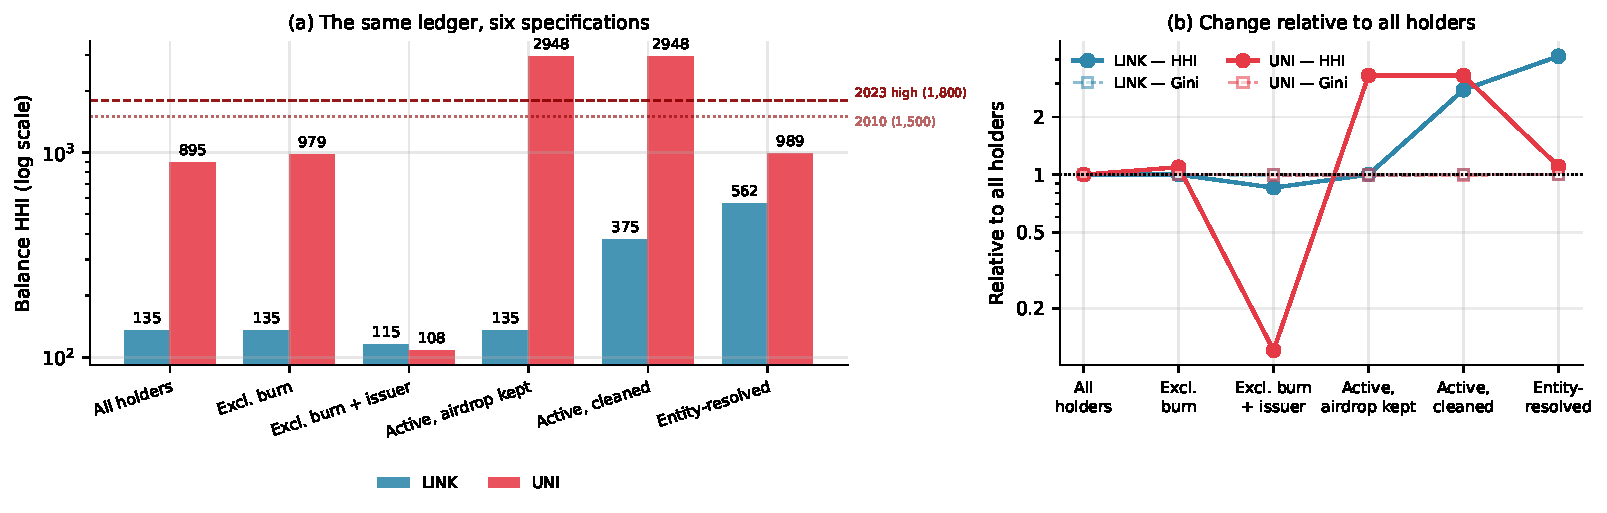
\includegraphics[width=0.95\linewidth]{fig_specification.pdf}
  \caption{Balance concentration of the same snapshot under six
  specifications. (a) HHI on a logarithmic scale; dashed line: 2023 threshold
  (1{,}800), dotted: 2010 moderate threshold (1{,}500). ``Active, airdrop
  kept'' and ``Active, cleaned'' differ only in whether the dust-airdrop
  transfers count as activity. (b) HHI and Gini relative to the all-holder
  specification: over these six specifications the HHI moves by an order of
  magnitude on UNI while the Gini stays near the unit line. The balance floors
  of Table~\ref{tab:spec}, which act on the other end of the distribution and
  move the Gini instead, are not shown.}
  \label{fig:specification}
\end{figure*}

\paragraph{Balance concentration: which end of the distribution each choice
moves}
On UNI the balance HHI runs from \V{uni.hhi.min} to \V{uni.hhi.max} across the
rows of Table~\ref{tab:spec} (Fig.~\ref{fig:specification}), a factor of \V{uni.hhi.ratio}; the lower end is
reached by excluding the burn address and the issuer, the upper end by
restricting the population to transfer-active addresses, \V{uni.active_share}
of all holders, among which the governance timelock dominates. On LINK the
range is \V{link.hhi.min}--\V{link.hhi.max}. These are the extremes of
varying one choice at a time. Over the eighteen combinations of population,
address type and entity resolution in Table~\ref{tab:combos} the UNI range
widens to \V{combo.uni.nf_hhi_min}--\V{combo.uni.nf_hhi_max}, the maximum
reached by combining the transfer-active population with entity resolution;
the LINK range is \V{combo.link.nf_hhi_min}--\V{combo.link.nf_hhi_max}. Over
the same eighteen the balance Gini moves by at most
\V{combo.link.gini_range_nofloor} on LINK and
\V{combo.uni.gini_range_nofloor} on UNI.

Varying one choice with the other two held fixed separates three kinds of
choice. \emph{Address type and entity resolution act on the top.} They
remove or merge a handful of large holders, change the HHI by up to a
factor of \V{fx.top.hhi_max} on either ledger and the Gini by at most
\V{fx.top.gini_max}. \emph{A balance floor acts on the tail.} Counting only
holdings of at least 0.01 tokens, or of at least USD~100 at the snapshot price
(\V{link.vfloor} LINK and \V{uni.vfloor} UNI, from the Chainlink price
feeds at the snapshot block), keeps \V{link.n.dust} and \V{link.n.value} of
the \V{link.holders} LINK holders and \V{uni.n.dust} and \V{uni.n.value} of
the \V{uni.holders} UNI holders. The value floor lowers the Gini by
\V{link.gini.drop_value} on LINK and \V{uni.gini.drop_value} on UNI; read as
$1-\mathrm{Gini}$, the distance from perfect inequality, that is a rise from
\V{link.omg.all} to \V{link.omg.value} (\V{link.omg.ratio}-fold) and from
\V{uni.omg.all} to \V{uni.omg.value} (\V{uni.omg.ratio}-fold). Neither
floor changes the HHI by more than \V{floor.hhi_change_max} in any cell of
the grid. \emph{Restricting to transfer-active addresses acts on both ends}:
it drops inactive large holders as well as the dormant tail, and changes the
HHI by up to a factor of \V{fx.link.activity.hhi} on LINK and
\V{fx.uni.activity.hhi} on UNI and the Gini by up to
\V{fx.link.activity.gini} and \V{fx.uni.activity.gini}. On LINK that Gini
change is more than half the value floor's (\V{fx.link.floor.gini} at most),
which is why the eighteen-cell Gini range is not small relative to the
floors. The HHI is a sum of squared shares and responds to how the largest
few participants are defined; the Gini is a function of the whole
distribution and responds to how many small holders are counted. Reporting
one does not report the other, and a population choice moves both.

For flows, averaging thirteen weekly values gives \V{link.fhhi.ratio_pooled}
(LINK) and \V{uni.fhhi.ratio_pooled} (UNI) times the HHI of the pooled 90-day
flow, because pooling averages away the week-to-week entry and exit of the
largest senders. The direction of the flow makes almost no difference.

\paragraph{Classifications that change}
Under the 2023 threshold, one row of Table~\ref{tab:spec} changes the
classification: restricting UNI to transfer-active holders, which places it
above 1{,}800 (and above 2{,}500 under the 2010 convention). No mean flow
figure on either ledger reaches 1{,}800. Among individual weeks, LINK's
largest address-level flow HHI is \V{link.fhhi.max} and its largest
entity-resolved week \V{link.fhhi.entity_max}; UNI's are \V{uni.fhhi.max} and
\V{uni.fhhi.entity_max}. Under the 2010 convention LINK's entity-resolved
maximum lies in the moderately concentrated band (above 1{,}500); under the
2023 convention, which has no moderate band, every week of both ledgers is
below the threshold.

\paragraph{The burn address raises the HHI when it is removed}
Excluding the UNI burn address, which holds \V{uni.burn_pct} of supply,
\emph{raises} the balance HHI from \V{uni.hhi.all} to \V{uni.hhi.excl_burn}.
Removing a participant with share $s_b$ removes $(100 s_b)^2$ points but
rescales every remaining squared share by $1/(1-s_b)^2$, and here the second
effect dominates.

\paragraph{Cleaning is a specification}
The transfer-active population depends on what counts as a transfer. On LINK
the dust airdrop of Section~\ref{sec:airdrop} reached most holders, so with
the airdrop transfers kept, \V{link.active_noair} addresses are
transfer-active, \V{link.nh.active_noair} of them with a positive balance, and
the HHI of those balances is \V{link.hhi.active_noair}, indistinguishable from
the all-holder figure; with them removed, \V{link.active} addresses remain
active, \V{link.nh.active} of them holders, and the HHI is
\V{link.hhi.active}. A
first-version statement that LINK's population choice was ``immaterial''
was an artefact of the airdrop. The airdrop went to existing holders rather
than creating dust-only addresses: the \V{link.airdrop_only.n} holders whose
only transfers in the window are airdrop receipts have a median balance of
\V{link.airdrop_only.med} LINK, and \V{link.airdrop_only.dust} of them hold
less than the 0.01-token dust floor. Flow concentration, being value-weighted, is
unaffected by \V{link.airdrop_total_link_short} LINK of dust.

\subsection{What the published literature uses}
\label{sec:lit}
Table~\ref{tab:lit} records the specification choices of the studies closest
to ours. None of them is wrong; they are different measurements, and their
numbers are comparable only after the choices are aligned.

\begin{table*}[t]
\centering\footnotesize
\caption{Specification choices in related studies, from the papers
themselves.}
\label{tab:lit}
\setlength{\tabcolsep}{4pt}
\begin{tabular}{@{}>{\raggedright}p{2.7cm}>{\raggedright}p{2.3cm}>{\raggedright}p{4.4cm}>{\raggedright}p{3.6cm}>{\raggedright\arraybackslash}p{3.0cm}@{}}
\toprule
Study & Quantity & Population / unit & Entity resolution & Aggregation \\
\midrule
Srinivasan \& Lee \cite{srinivasan2017quantifying} & Gini, Nakamoto & Addresses with $\geq$185 BTC or $\geq$2,477 ETH (about USD 500,000 in July 2017) & --- & Snapshot \\
Sai et al.\ \cite{sai2021wealth} & Balance Gini & All addresses with a balance (a USD 100 floor, attributed to \cite{srinivasan2017quantifying}, discussed but not applied) & ML clustering for Bitcoin only & Time series \\
Nadler \& Sch\"ar \cite{nadler2022defi} & Top-$n$, Gini & 500 largest holders & Custodial contracts mapped to beneficiaries & Snapshots \\
Lin et al.\ \cite{lin2021measuring} & Gini, entropy, Nakamoto & Mining pools & --- & Day / week / month, fixed and sliding \\
Fritsch et al.\ \cite{fritsch2024voting} & Gini, Nakamoto & Holders vs.\ delegates vs.\ voting delegates & --- & Snapshot \\
This paper & HHI, Gini, Nakamoto & All of Table~\ref{tab:spec} & Label-based, lower bound & Weekly mean and pooled \\
\bottomrule
\end{tabular}
\end{table*}

\subsection{A reporting checklist}
\label{sec:checklist}
Two on-chain concentration figures are comparable only if they agree on the
following, each of which moves at least one statistic in
Table~\ref{tab:spec}:
\begin{enumerate}
  \item the balance snapshot (block or time) and the observation window;
  \item the holder population (all positive balances, transfer-active, top
  $n$) and any balance floor;
  \item the address types excluded (burn, issuer, protocol contracts) and how
  they were identified;
  \item the unit of analysis (address or entity) and, if entities, the label
  source, its retrieval date and its coverage;
  \item for flows, the temporal aggregation and the direction;
  \item the cleaning rules (mint/burn, zero-value, spam or airdrops), with
  the number of records each removes;
  \item for anything computed on a graph, how repeated transfers between a
  pair are aggregated;
  \item for governance, whether weight is balance or delegated votes, and the
  thresholds as read from the contract.
\end{enumerate}

\subsection{Reference points}
\label{sec:benchmarks}
For orientation, Fig.~\ref{fig:hhi} places our figures beside three
reference markets whose HHI we could compute or source exactly. The national
U.S.\ deposit market, with deposits aggregated to the top-tier holding company
from the FDIC Summary of Deposits at 30 June 2026, has an HHI of
\V{bench.us_bank} \cite{fdic2026sod}; the European Central Bank reports
\V{bench.sweden} for the total assets of Swedish credit institutions in
\V{bench.sweden_year} \cite{ecb2026ssi}; and the purchase volumes of the four
largest global card networks in 2022, as published by the Nilson Report,
imply an HHI of \V{bench.cards} \cite{nilson2023issue1241}, taking shares of
the six global brands' combined volume (\V{bench.cards_top4} if the four are
taken as the whole market). National
aggregates understate the concentration of the local markets in which banks
compete, so these points indicate magnitude only. Routing on both ledgers is
of the same order as national U.S.\ deposit-taking and an order of magnitude
below card networks.

\begin{figure}[t]
  \centering
  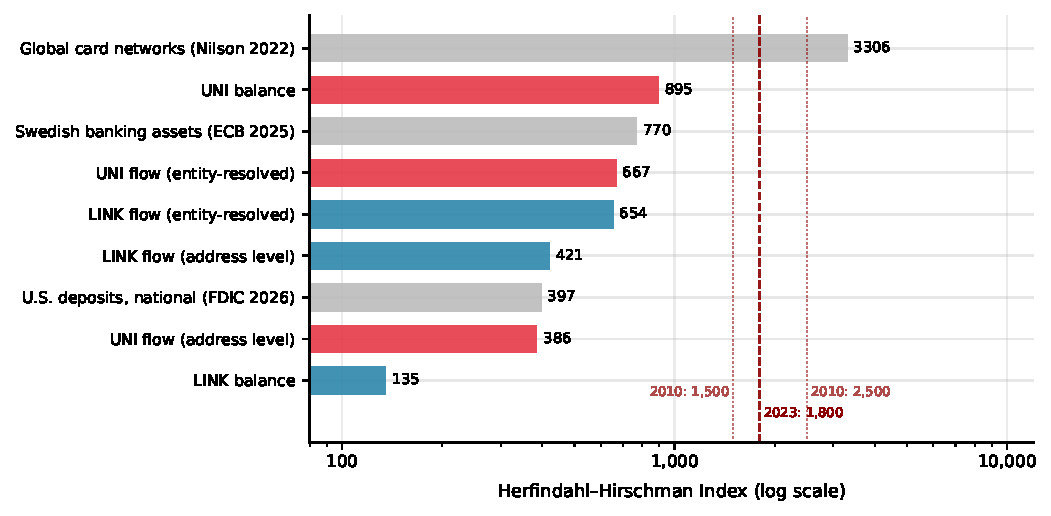
\includegraphics[width=\linewidth]{fig_hhi_benchmark.pdf}
  \caption{HHI on a logarithmic scale: balance and weekly flow concentration
  for both ledgers at address level and after label-based entity resolution,
  beside three reference markets (FDIC Summary of Deposits 2026; ECB
  structural financial indicators; Nilson Report Issue 1241). Dashed line:
  2023 Merger Guidelines threshold (1{,}800); dotted lines: 2010 thresholds
  (1{,}500 and 2{,}500). The comparison is an analogy of magnitude, not an
  application of the guidelines.}
  \label{fig:hhi}
\end{figure}

\subsection{An implementation choice that changes downstream results}
\label{sec:edgecase}
Repeated transfers between an ordered pair must be summed into one weighted
edge (Eq.~\eqref{eq:edgeweight}). Building the graph with
\texttt{networkx.from\_pandas\_edgelist(\ldots, create\_using=nx.DiGraph())}
instead keeps the last record of each pair and raises no error; node set,
edge set and degree sequence are unchanged. On the $10^{4}$ subgraphs this
discards \V{link.ew.loss_1w} (LINK) and \V{uni.ew.loss_1w} (UNI) of
transferred volume. PageRank computed the two ways has a Pearson correlation of
\V{link.ew.corr_1w} and \V{uni.ew.corr_1w}, and the fifty highest-ranked
addresses coincide in \V{link.ew.top50_1w} and \V{uni.ew.top50_1w} of fifty
positions.

We reran the whole pipeline with overwritten edges and nothing else changed
(Table~\ref{tab:edgecase}). The hidden-broker sets grow and change
membership, and the
number of brokers shared by the two ledgers goes from \V{ew.shared.main} to
\V{ew.shared.overwrite}. The classical-centrality AUC is lower with
overwritten edges, but a paired node bootstrap over pooled out-of-fold
predictions puts the difference at
\V{aci.link.cent_ow} (95\% CI \V{aci.link.cent_ow.ci}) on LINK and
\V{aci.uni.cent_ow} (\V{aci.uni.cent_ow.ci}) on UNI, so we do not read
anything into it. Weekly flow concentration moves too (\V{link.fhhi.weekly} to \V{link.fhhi.overwrite} on LINK), because
it is computed from the weighted out-degree of each weekly graph. The error is
invisible to every check that does not involve weights.

The first version of this paper attributed a further effect to this choice:
under the superseded pipeline the infrastructure cluster had a median
balance of \V{v16.core.medbal}, which had supported a contrast between the
two tokens that the corrected pipeline removed. Isolating edge aggregation
does not reproduce that result---with overwritten edges the infrastructure
cluster has a median balance of \V{ew.link.overwrite.coremedbal} against
\V{ew.link.main.coremedbal} with summed edges---so the earlier contrast
also reflected other differences between the superseded and the corrected
pipeline. We retract the attribution, not the correction: the summed
construction is the right one, and the effects in Table~\ref{tab:edgecase}
are reproducible from the archived code. We have not isolated which of the
other differences in the superseded pipeline produced the earlier contrast.

\begin{table*}[t]
\centering\small
\caption{The same pipeline with summed and with overwritten edge weights
(main cleaning specification). Rows other than the last use the $10^{4}$
subgraphs; the weekly flow HHI is computed on all cleaned transfers. Purity
ratio: neighbourhood purity of core nodes in the GraphSAGE embedding divided by
that in the structural features (\ref{app:instrument}). Brokers: set size /
overlap with the summed-edge set. AUC: fold-averaged as in
Table~\ref{tab:instrument}, and pooled over out-of-fold predictions, the
basis of the paired bootstrap in the text.}
\label{tab:edgecase}
\setlength{\tabcolsep}{3.5pt}
\begin{tabular}{@{}lcccc@{}}
\toprule
& \multicolumn{2}{c}{LINK} & \multicolumn{2}{c}{UNI} \\
\cmidrule(lr){2-3}\cmidrule(l){4-5}
& Summed & Overwritten & Summed & Overwritten \\
\midrule
Centrality AUC (fold avg.) & \V{ew.link.main.cent} & \V{ew.link.overwrite.cent} & \V{ew.uni.main.cent} & \V{ew.uni.overwrite.cent} \\
Centrality AUC (pooled) & \V{aci.link.pool.cent} & \V{aci.link.pool.cent_ow} & \V{aci.uni.pool.cent} & \V{aci.uni.pool.cent_ow} \\
GraphSAGE AUC (fold avg.) & \V{ew.link.main.gnn} & \V{ew.link.overwrite.gnn} & \V{ew.uni.main.gnn} & \V{ew.uni.overwrite.gnn} \\
Purity ratio & \V{ew.link.main.purratio} & \V{ew.link.overwrite.purratio} & \V{ew.uni.main.purratio} & \V{ew.uni.overwrite.purratio} \\
Core cluster med.\ balance & \V{ew.link.main.coremedbal} & \V{ew.link.overwrite.coremedbal} & \V{ew.uni.main.coremedbal} & \V{ew.uni.overwrite.coremedbal} \\
Brokers & \V{ew.link.main.brokers} & \V{ew.link.overwrite.brokers} / \V{ew.link.overwrite.overlap} & \V{ew.uni.main.brokers} & \V{ew.uni.overwrite.brokers} / \V{ew.uni.overwrite.overlap} \\
Weekly flow HHI & \V{link.fhhi.weekly} & \V{link.fhhi.overwrite} & \V{uni.fhhi.weekly} & \V{uni.fhhi.overwrite} \\
\bottomrule
\end{tabular}
\end{table*}

% =========================================================================
\section{Hidden Brokers and What Selects Them (RQ2)}
\label{sec:brokers}

\subsection{Scoring structural position}
\label{sec:instrument}
The criterion needs a score $s$ of structural centrality that works on a
ledger where most addresses carry no label. We obtain it by predicting the
\emph{core} label of Section~\ref{sec:data} from structure alone: a logistic
regression (standardised inputs, balanced class weights) evaluated by
stratified five-fold cross-validation with shuffling. The label never enters
the inputs. Table~\ref{tab:instrument} compares four inputs, and a constant-input control, on the $10^{4}$
subgraphs: PageRank and sampled betweenness alone; the seven hand-crafted
structural features of Section~\ref{sec:data}; and two learned
16-dimensional embeddings, an unsupervised two-layer GraphSAGE encoder
\cite{hamilton2017inductive} (hidden width 32, 200 epochs, Adam with learning
rate 0.01, link-reconstruction objective with negative sampling) and
node2vec. Learned embeddings are averaged over independent initialisations.

\begin{table}[t]
\centering\small
\caption{Cross-validated AUC for predicting the core label from structure
($10^{4}$ subgraphs). Fold avg.: mean of the five fold AUCs (GNN: mean
$\pm$ s.d.\ over ten initialisations; node2vec: five). Pooled: one AUC over
all out-of-fold predictions, the basis of the bootstrap intervals in the
text; for GraphSAGE the median over the ten single-seed models, and a
separate row for the ten-seed ensemble. Differences quoted in the text are
computed before rounding. Anchors: number of core-labelled nodes.}
\label{tab:instrument}
\setlength{\tabcolsep}{3pt}\footnotesize
\begin{tabular}{@{}lcccc@{}}
\toprule
& \multicolumn{2}{c}{LINK} & \multicolumn{2}{c}{UNI} \\
\cmidrule(lr){2-3}\cmidrule(l){4-5}
Input & Fold avg. & Pooled & Fold avg. & Pooled \\
\midrule
PageRank + betw. & \V{c1.link.cent} & \V{aci.link.pool.cent} & \V{c1.uni.cent} & \V{aci.uni.pool.cent} \\
Structural features (7) & \V{c1.link.struct} & \V{aci.link.pool.struct} & \V{c1.uni.struct} & \V{aci.uni.pool.struct} \\
GraphSAGE, single seed & \V{c1.link.gnn} & \V{aci.link.pool.gnn_single} & \V{c1.uni.gnn} & \V{aci.uni.pool.gnn_single} \\
GraphSAGE ensemble & --- & \V{aci.link.pool.gnn_ens} & --- & \V{aci.uni.pool.gnn_ens} \\
node2vec & \V{c1.link.n2v} & --- & \V{c1.uni.n2v} & --- \\
GraphSAGE, const.\ input & \V{c1.link.nofeat} & --- & \V{c1.uni.nofeat} & --- \\
\midrule
Nodes / anchors & \multicolumn{2}{c}{\V{link.nodes.1w} / \V{link.anchors.1w}} & \multicolumn{2}{c}{\V{uni.nodes.1w} / \V{uni.anchors.1w}} \\
\bottomrule
\end{tabular}
\end{table}

The gap that matters is between the two-feature centrality baseline and
everything else. The seven structural features, which include degree and
counterparty count, recover the label nearly as well as either learned
embedding; the GraphSAGE embedding exceeds them by \V{c1.link.gnn_margin} on
LINK and \V{c1.uni.gnn_margin} on UNI in fold-averaged AUC. With only
\V{link.anchors.1w} and \V{uni.anchors.1w} positives, seed-level standard
deviations understate the uncertainty, so we also bootstrap nodes over pooled
out-of-fold predictions (Table~\ref{tab:instrument}, pooled columns). The
structural features beat centrality by \V{aci.link.struct_cent} (95\% CI
\V{aci.link.struct_cent.ci}) on LINK and \V{aci.uni.struct_cent}
(\V{aci.uni.struct_cent.ci}) on UNI. The ten-seed GraphSAGE ensemble beats
the structural features by \V{aci.link.gnn_struct}
(\V{aci.link.gnn_struct.ci}) and \V{aci.uni.gnn_struct}
(\V{aci.uni.gnn_struct.ci}), only just distinguishable from zero. Part of
that margin is the ensemble rather than the representation: the structural
features are a single model, and a single GraphSAGE model beats them by a
median \V{aci.link.single.diff} on LINK (\V{aci.link.single.range} across
seeds) and \V{aci.uni.single.diff} on UNI (\V{aci.uni.single.range}), with
the 95\% interval excluding zero for \V{aci.link.single.nexcl} and
\V{aci.uni.single.nexcl} of the ten seeds respectively. What separates good from poor
inputs is therefore mainly whether they contain degree and counterparty
information, not whether they are learned.
Replacing all inputs with a constant collapses the GraphSAGE embedding to
chance, a degeneracy of mean aggregation over uninformative inputs; node2vec,
which uses topology alone, shows that topology is informative. On the
$5\times10^{4}$ and full LINK graphs the ordering is the same
(\ref{app:instrument}). We use the GraphSAGE score as $s$ and treat that
choice as a parameter.

\subsection{The criterion}
\label{sec:criterion}
A node is a hidden broker if (i) its score $s$ is in the top 1\%, (ii) its
balance is at most the median balance of the subgraph, (iii) it has
at least five distinct counterparties, (iv) its sampled betweenness is
positive, and (v) it is unlabelled in the archived compilation. Conditions
(iii) and (iv) exclude addresses that cannot sit on any path. Because a hard
percentile cut is sensitive to initialisation, $s$ is the mean percentile
rank over ten independently initialised embeddings, cut once.
The median in condition (ii) is zero on UNI, where \V{uni.zero_share} of the
subgraph's nodes hold nothing, and \V{link.med_bal} LINK on LINK, where
\V{link.zero_share} hold nothing and the median node holds a residue of order
$10^{-5}$ tokens. Condition (ii) therefore admits zero or
dust balances: \V{link.brokers_zero_bal} of the LINK brokers and
\V{uni.brokers_zero_bal} of the UNI brokers hold exactly zero
(Table~\ref{tab:brokerspec} gives the sets under a strict zero-balance
condition and under a 0.01-token dust floor).

Under the main specification the criterion selects \V{link.brokers} addresses
on LINK and \V{uni.brokers} on UNI, \V{shared.brokers} of them on both. An
alternative rule---selection in at least half of the ten individual runs---gives
\V{link.brokers_vote} and \V{uni.brokers_vote}, and the two rules agree on
\V{link.brokers_both} and \V{uni.brokers_both}. A betweenness-based selection
of the same size from the same pool shares \V{link.brokers_bet_overlap} and
\V{uni.brokers_bet_overlap} addresses with the GraphSAGE selection.

\subsection{What the selected set depends on}
\label{sec:stability}
\paragraph{Initialisation}
Training is deterministic for a given seed (\ref{app:repro}); across the ten
seeds, \V{link.brokers_ever} LINK addresses are selected at least once and
\V{link.brokers_rare} of them at most twice, which is why we report the rank
ensemble rather than a single run.

\paragraph{Data cleaning}
The selected set moves with the cleaning specification
(Table~\ref{tab:brokerspec}). Of the \V{v1.link.brokers} LINK and
\V{v1.uni.brokers} UNI brokers reported in the first version of this paper,
which used uncleaned transfers, \V{link.brokers_v1_kept} and
\V{uni.brokers_v1_kept} remain, and the number shared by the two ledgers
falls from \V{v1.shared.brokers} to \V{shared.brokers}. The causes differ by
ledger. On LINK the change is mainly the cleaning: with both cleaning rules
switched off, the present pipeline recovers \V{link.brokers_v1_raw} of the
first version's \V{v1.link.brokers}. On UNI, where cleaning removes almost
nothing and every cleaning specification gives the same set
(Table~\ref{tab:brokerspec}), the change comes from the end-of-window balance
snapshot and from the determinism corrections of \ref{app:repro}: only
\V{uni.brokers_v1_raw} of the first version's \V{v1.uni.brokers} are
recovered even without cleaning. With the airdrop transfers kept, the LINK set
has \V{spec.link.brokers.keep_airdrop} members, of which
\V{spec.link.overlap.keep_airdrop} are in the main set; with zero-value
transfers kept it has \V{spec.link.brokers.keep_zero}
(\V{spec.link.overlap.keep_zero} shared). On UNI, where the airdrop rule
removes nothing, keeping zero-value transfers alone gives a set of
\V{spec.uni.brokers.keep_zero}, of which \V{spec.uni.overlap.keep_zero} are in the main set.

\begin{table}[t]
\centering\small
\caption{Hidden-broker sets under the cleaning specifications of
\ref{app:cleaning} and under two alternative balance conditions (ii): size,
and overlap with the main set. Balance-condition rows reuse the main
ensemble scores; the addresses they add to the main set (\V{bsens.link.dust.new} on
LINK and \V{bsens.uni.dust.new} on UNI under the dust condition) were not verified.}
\label{tab:brokerspec}
\begin{tabular}{@{}lcccc@{}}
\toprule
& \multicolumn{2}{c}{LINK} & \multicolumn{2}{c}{UNI} \\
\cmidrule(lr){2-3}\cmidrule(l){4-5}
Specification & Size & Overlap & Size & Overlap \\
\midrule
\textbf{Main} & \V{link.brokers} & --- & \V{uni.brokers} & --- \\
Zero-value kept & \V{spec.link.brokers.keep_zero} & \V{spec.link.overlap.keep_zero} & \V{spec.uni.brokers.keep_zero} & \V{spec.uni.overlap.keep_zero} \\
Airdrop kept & \V{spec.link.brokers.keep_airdrop} & \V{spec.link.overlap.keep_airdrop} & \V{spec.uni.brokers.keep_airdrop} & \V{spec.uni.overlap.keep_airdrop} \\
Both kept & \V{spec.link.brokers.raw} & \V{spec.link.overlap.raw} & \V{spec.uni.brokers.raw} & \V{spec.uni.overlap.raw} \\
Edges overwritten & \V{spec.link.brokers.overwrite} & \V{spec.link.overlap.overwrite} & \V{spec.uni.brokers.overwrite} & \V{spec.uni.overlap.overwrite} \\
\addlinespace[2pt]
\multicolumn{5}{@{}l}{\emph{Balance condition (main data)}} \\
Balance exactly zero & \V{bsens.link.zero.size} & \V{bsens.link.zero.overlap} & \V{bsens.uni.zero.size} & \V{bsens.uni.zero.overlap} \\
Balance $<$ 0.01 tokens & \V{bsens.link.dust.size} & \V{bsens.link.dust.overlap} & \V{bsens.uni.dust.size} & \V{bsens.uni.dust.overlap} \\
\bottomrule
\end{tabular}
\end{table}

\paragraph{Representation}
node2vec, scored and cut in the same way, selects \V{link.n2v_brokers} LINK
addresses, of which \V{link.n2v_overlap} are also in the GraphSAGE set. Among
its top percentile \V{link.n2v_top1_labelled} of nodes carry a label, against
\V{link.gnn_top1_labelled} for GraphSAGE: node2vec ranks catalogued
infrastructure highest, and that infrastructure is removed by condition (v).

\subsection{Does the representation add anything? A matched control}
\label{sec:control}
That the selected addresses turn out to be routing infrastructure does not by
itself show the selection was informative, since we inspected only what it
chose. We therefore drew controls from the same eligibility pool---conditions
(ii)--(v) without (i)---restricted to addresses not selected, and verified
them blind. The pool's median counterparty count is \V{ctl.pool_med_cp}
against \V{ctl.broker_med_cp} for the brokers, so an unmatched control would
differ in degree as well as in selection; the main control matches each of 20
brokers, drawn at random, to the unselected address closest in counterparty
count. Group sizes (20 matched, 10 unmatched, 8 broker anchors) and the random
seed were fixed in advance, sized to detect a difference of 30 percentage
points (35\% against 5\%) with a one-sided Fisher test; at the observed
matched-control rate, 80\% power at $\alpha = 0.05$ requires a difference of
about \V{ctl.mdd} points. Controls, anchors and
any broker without an earlier verification record were shuffled into one list
without group labels and verified by one author; addresses verified in the
first version of this paper keep that record. Verification uses Etherscan
name tags, verified source and deployer, and the token-transfer history, and
assigns one of: a named protocol, an unlabelled routing contract, an MEV bot,
or unknown. Centralized-exchange deposit and hot-wallet addresses are not
routing protocols and are scored as unknown; we fixed this rule before
unblinding, and it changes only the unmatched group
(\ref{app:control}).

The blinded anchors were judged exactly as in the earlier record
(\V{ctl.anchor_agree} anchors), and resolve to named protocols at
\V{ctl.anchor_pct} against \V{ctl.broker_pct} for all brokers, so the standard
did not shift under blinding. Of the 20 matched controls, \V{ctl.matched_k}
(\V{ctl.matched_pct}, 95\% CI \V{ctl.matched_ci}) resolve to a named protocol,
against \V{ctl.broker_k} of \V{link.brokers} brokers (\V{ctl.broker_pct},
\V{ctl.broker_ci}); one-sided Fisher exact $p = \V{ctl.p}$. Of the ten
unmatched controls, \V{ctl.uniform_k} do (\V{ctl.uniform_pct},
\V{ctl.uniform_ci}); the difference between matched and unmatched controls is
in the expected direction but not significant ($p = \V{ctl.p_mu}$).

\begin{figure}[t]
  \centering
  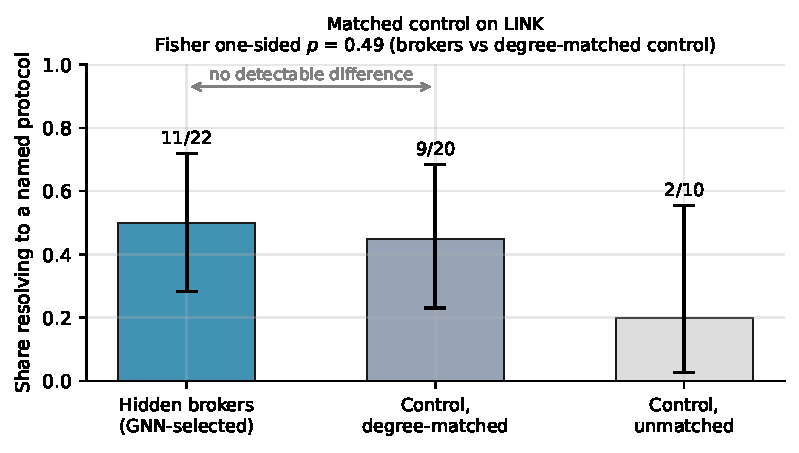
\includegraphics[width=\linewidth]{fig_random_control.pdf}
  \caption{Matched control on LINK: share of each group resolving to a named
  routing protocol under blind verification, with Clopper--Pearson 95\%
  intervals. Matched controls come from the same eligibility pool as the
  brokers and are matched on counterparty count.}
  \label{fig:control}
\end{figure}

Conditional on counterparty count, then, the learned score adds nothing we
can detect (Fig.~\ref{fig:control}). The 95\% interval for the difference between brokers and matched
controls is \V{ctl.diff_ci} percentage points: it excludes an advantage of
more than about a third, but not a small one, so the defensible statement is
that no advantage was detected. Either way, the finding that these addresses are
routing infrastructure does not depend on the representation used to surface
them.

\subsection{Verification and live labels}
\label{sec:verify}
Every address in the union of the two broker sets (\V{brokers.union}
addresses) has a manual verification record, and \V{brokers.union_named}
resolve to a named protocol: DEX aggregators and swap routers, intent
solvers, wallet swap interfaces and cross-chain routers. ``Unlabelled'' is
relative to the archived compilation, not to the block explorer: checked on
6 October 2026, \V{brokers.live_tagged} of the \V{brokers.union} carry an
Etherscan public name tag and \V{brokers.live_untagged} do not. The
compilation's gaps are largely a matter of age. Of the \V{deploy.n_contracts}
contracts among the brokers (the remaining address is an exchange wallet),
\V{deploy.n_after} were deployed after the compilation was last scraped in
June 2023; the other two, MetaMask's swap spender (2020) and LI.FI's router
(2022), predate it and are missing anyway. A hidden broker is therefore, for
the most part, routing infrastructure newer than the label set used to look
for it, and the criterion is best read as a way of finding what a dated label
set misses. Of the \V{shared.brokers} addresses selected on both
ledgers, \V{shared.brokers_named} are named protocols
(\V{shared.brokers_names}); the remaining one is an unlabelled routing
contract. Structural coreness is agnostic to legitimacy:
the union also contains MEV bots and a centralized-exchange hot wallet absent
from the compilation, so the signature---many counterparties, no
custody---identifies operational centrality, not role or intent.

% =========================================================================
\section{Ownership, Routing and Rules (RQ3)}
\label{sec:layers}

\subsection{Ownership and routing are weakly related}
\label{sec:wealth-power}
Both ledgers are extremely unequal in ownership---balance Gini
\V{link.gini.all} and \V{uni.gini.all}, with the top 1\% of addresses holding
\V{link.top1} and \V{uni.top1} of supply---yet unconcentrated in routing,
with a mean weekly flow HHI of \V{link.fhhi.weekly} and \V{uni.fhhi.weekly}.
Across the addresses of the $10^{4}$ subgraph that hold a positive balance,
the rank correlation between balance and counterparty count is
\V{link.rho.cp.pos} on LINK ($n = \V{link.rho.n.pos}$, 95\% CI
\V{link.rho.cp.pos.ci}) and \V{uni.rho.cp.pos} on UNI
($n = \V{uni.rho.n.pos}$, \V{uni.rho.cp.pos.ci}); between balance and
betweenness it is \V{link.rho.bet.pos} (\V{link.rho.bet.pos.ci}) and
\V{uni.rho.bet.pos} (\V{uni.rho.bet.pos.ci}). Including the addresses with
zero balance gives \V{link.rho.cp.all}
and \V{uni.rho.cp.all} for counterparties. These correlations are small in
magnitude; with samples of this size some are nonetheless distinguishable
from zero, and we read them as weak association rather than independence.
Weak association is what allows extreme ownership inequality to coexist with
an unconcentrated routing layer: knowing who holds the supply says little
about who moves it.

\subsection{The rule layer, measured in delegated votes}
\label{sec:governance}
Uniswap governance is a threshold game. Submitting an on-chain proposal
requires $10^{6}$ UNI of votes delegated to the proposer, and a proposal
passes with $4\times10^{7}$ UNI of votes in favour
\cite{uniswap2026governance}; we read both values from the governor contract
at the first and last block of the window. Votes are not balances. A token
carries voting weight only once its holder delegates it, to itself or to
another address, and the weight is checkpointed per block. We therefore
measure the rule layer in delegated votes at the snapshot block, read from
the token contract: we query the delegate of every one of the \V{uni.holders}
holders and the checkpointed votes of every one of the
\V{uni.gov.n_delegates} delegates, and verify that each delegate's votes
equal the summed balance of the holders delegating to it.

\paragraph{Specification again}
Table~\ref{tab:gov} sets the delegated-vote measurement beside the
balance-based one used in the first version of this paper.
\V{uni.gov.deleg_share} of the supply was delegated at the snapshot. Counting
balances, the smallest set of voting-capable addresses holding $4\times10^{7}$
UNI has \V{uni.gov.bal.nonvoting.n_quorum} members; the two addresses in
question are a Binance hot wallet and an unlabelled address
(\V{uni.gov.nonvoting.m2}), and neither has delegated, so their voting weight
is zero. Excluding custodial addresses as well removes the Binance wallet;
its place is taken by a second unlabelled address
(\V{uni.gov.custodial.m2}), which has not delegated either. Counting delegated votes,
\V{uni.gov.n_quorum} delegates are needed to reach the quorum and
\V{uni.gov.n_half} to hold a majority of all delegated votes---close to the
eleven that Fritsch et al.\ report for Uniswap in March 2022
\cite{fritsch2024voting}. \V{uni.gov.n_eligible} delegates individually hold
enough votes to submit a proposal. A balance-based count thus overstates
concentration in this instance, and the direction of the error is not
knowable in advance: it depends on who delegates.

\begin{table}[t]
\centering\small
\caption{The UNI rule layer under four specifications at block
\V{snapshot.block}. $N_{40\mathrm{M}}$: fewest addresses whose combined weight
reaches the $4\times10^{7}$ UNI quorum. $N_{50\%}$: fewest addresses holding
half of the total weight. $\geq 1\mathrm{M}$: addresses that individually
meet the proposal threshold. Only delegated votes carry voting weight.}
\label{tab:gov}
\setlength{\tabcolsep}{3.5pt}
\begin{tabular}{@{}lcccc@{}}
\toprule
Specification & $N_{40\mathrm{M}}$ & $N_{50\%}$ & $\geq 1\mathrm{M}$ & Weight / supply \\
\midrule
Balances, all holders & \V{uni.gov.bal.all.n_quorum} & \V{uni.gov.bal.all.n_half} & \V{uni.gov.bal.all.n_eligible} & \V{uni.gov.bal.all.share} \\
Balances, excl.\ non-voting & \V{uni.gov.bal.nonvoting.n_quorum} & \V{uni.gov.bal.nonvoting.n_half} & \V{uni.gov.bal.nonvoting.n_eligible} & \V{uni.gov.bal.nonvoting.share} \\
\quad and excl.\ custodial & \V{uni.gov.bal.custodial.n_quorum} & \V{uni.gov.bal.custodial.n_half} & \V{uni.gov.bal.custodial.n_eligible} & \V{uni.gov.bal.custodial.share} \\
\textbf{Delegated votes} & \textbf{\V{uni.gov.n_quorum}} & \textbf{\V{uni.gov.n_half}} & \textbf{\V{uni.gov.n_eligible}} & \V{uni.gov.deleg_share} \\
\bottomrule
\end{tabular}
\end{table}

\paragraph{The rule layer has already rewritten the routing layer}
On 25 December 2025 Uniswap governance passed the ``UNIfication'' proposal,
which activated protocol fees on Uniswap v2 and selected v3 pools, routed
those fees to a \texttt{TokenJar} contract on each chain, and burned $10^{8}$
UNI from the treasury; the burn was executed on 28 December
\cite{theblock2025unification, cointelegraph2025burn, uniswap2026fees}.
Assets leave a \texttt{TokenJar} only through the releaser contract it
designates, and the jar's owner---on Ethereum, the governance timelock---can
change that releaser. Throughout our window the Ethereum jar's releaser was the
Firepit contract listed in Uniswap's deployment documentation
\cite{uniswap2026deployments}, which releases the accumulated fees to whoever
burns \V{uni.firepit.threshold} UNI; we read both values from the chain at
the first and last block of the window. Its effects are visible in our data.
All \V{uni.burn.n} UNI records that a naive pipeline would discard as
``burns'' are transfers to \texttt{0x\ldots dEaD}: \V{uni.burn.hi.n} in lots
of \V{uni.burn.lot_hi} UNI from \V{uni.burn.hi.senders} senders on
Ethereum; \V{uni.burn.lo.n} in lots of \V{uni.burn.lot_lo} UNI, of which
\V{uni.burn.lo.bridged} arrive through the Base, Arbitrum, Optimism and
Unichain bridges and \V{uni.burn.lo.other} from an unlabelled address---a lot
size that matches the \V{uni.burn.lot_lo}-UNI threshold we read at the end
of the window from the releasers on \V{uni.l2.chains}, each identified as
the address that the deployment page lists and that the chain's
\texttt{TokenJar} designates on chain (addresses and calls in the
repository, \ref{app:repro}); and one of \V{uni.burn.odd} UNI. They total \V{uni.burn.window} UNI. The burn address holds
\V{uni.burn_pct} of supply at the snapshot, of which $10^{8}$ UNI is the
one-off December burn. A vote of the rule layer changed the economics of
every swap routed through a fee-enabled pool, which is the strongest
evidence we have that routing contestability is held conditionally.

\paragraph{The rule layer and the routing layer do not overlap}
None of the \V{uni.gov.n_eligible} delegates that can submit a proposal is
among the 10, 50 or 100 largest senders of UNI by mean weekly outflow, and
\V{uni.gov.inactive} of them (\V{uni.gov.inactive_pct}) sent or received no
UNI at all during the window. The largest senders have delegated none of
their own balances. Because a hidden broker is defined to hold at most the
median balance, a comparison of brokers with proposal-eligible addresses
would be empty by construction; the outflow-based comparison has no balance
condition and could have found an overlap.

\paragraph{Routing under direct governance control}
Of mean weekly UNI outflow, \V{uni.gov.rev_l1} originates from contracts the
governance timelock controls and \V{uni.gov.rev_l2} from other
Uniswap-labelled contracts; \V{uni.gov.rev_l3} comes from addresses the label
compilation does not identify. This bounds direct control of UNI
\emph{token} routing, not of swap volume in Uniswap pools, which the fee
switch shows governance can reach.

LINK has no token-weighted governance: holding LINK confers no vote, and
while anyone may run a Chainlink oracle, each oracle network can restrict
which oracles contribute to it \cite{chainlink2022nodeoperator}. Of the two
ledgers whose routing layers we measure, only one has a rule layer that
token holders can use to change it.

% =========================================================================
\section{Case Study: A Coordinated Phishing Airdrop on LINK}
\label{sec:airdrop}

This section uses the uncleaned LINK records, because the event it describes
is what the cleaning rule of Section~\ref{sec:data} removes. In week
\V{airdrop.week} of the window LINK recorded \V{airdrop.week_tx} transfers,
\V{airdrop.week_ratio} times the median week. Of these,
\V{link.airdrop_tx}---all sent on \V{airdrop.days}---were transfers of
\V{airdrop.amt_lo} or \V{airdrop.amt_hi} LINK from \V{link.airdrop_senders} contracts to
\V{airdrop.recipients} distinct recipients, \V{airdrop.single_pct} of whom
received exactly one. The total value distributed was \V{airdrop.total_link}
LINK.

Our initial manual investigation, before the rule existed, identified \V{airdrop.archived_n}
contracts that expose an \texttt{Airdrop} method and present
themselves as ``LinkGiveaway'' or ``LinkStaking'', neither of which is a
Chainlink product; they account for exactly \V{airdrop.tx_archived}
transfers, \V{airdrop.per_contract} each. The rule recovers all \V{airdrop.archived_n} and
\V{airdrop.others} further senders responsible for the remaining
\V{airdrop.tx_others} transfers. We inspected each of the \V{airdrop.others}
on Etherscan: all are contracts that Etherscan flags as tokens ``reported for
impersonating well-known cryptocurrencies'', all were invoked through an
\texttt{Airdrop} method, and they were deployed by \V{airdrop.deployers}
addresses under names such as LinkEarn, LinkAward and BountyLink. The full
list, the funders identified in the initial investigation, and the Etherscan
classification as retrieved are archived with the code; we date the
classification because Etherscan labels can change.

The event separates two statistics that are often treated as
interchangeable (Table~\ref{tab:airdrop}). With the airdrop transfers
present, the receiver-side Gini of the week rises to \V{airdrop.gini_in_with}
from \V{airdrop.gini_in_without}; the sender-side flow HHI is
\V{airdrop.hhi_out_with} with and \V{airdrop.hhi_out_without} without them.
A flood of near-worthless transfers saturates an unweighted dispersion
measure over recipients while leaving value-weighted market structure
untouched. Its effect on structure is larger than on either statistic: the
airdrop adds \V{airdrop.addr_added} addresses to the week, enough to make
almost every LINK holder ``transfer-active'' and to change which addresses
enter the activity-ranked subgraphs (Table~\ref{tab:spec}).

\begin{table}[t]
\centering\small
\caption{LINK week \V{airdrop.week} with and without the airdrop transfers.
Both columns remove mint/burn and zero-value records; they differ only in
the airdrop rule.}
\label{tab:airdrop}
\begin{tabular}{@{}lrr@{}}
\toprule
 & With airdrop & Without \\
\midrule
Transfers & \V{airdrop.ntx_with} & \V{airdrop.ntx_without} \\
Addresses & \V{airdrop.naddr_with} & \V{airdrop.naddr_without} \\
Receiver-side Gini & \V{airdrop.gini_in_with} & \V{airdrop.gini_in_without} \\
Sender-side Gini & \V{airdrop.gini_out_with} & \V{airdrop.gini_out_without} \\
Sender-side flow HHI & \V{airdrop.hhi_out_with} & \V{airdrop.hhi_out_without} \\
\bottomrule
\end{tabular}
\end{table}

% =========================================================================
\section{Limitations}
\label{sec:limitations}

\textbf{Two ledgers.} Every result is replicated on two tokens, and holding
the window fixed removes market regime as a confound, but two ledgers cannot
establish how widely the specification ranges of Table~\ref{tab:spec} hold
across the asset class. The rule layer is measured on UNI only, because LINK
has no token-weighted governance.

\textbf{One window.} Ninety days include one coordinated phishing event but
not a full market cycle.

\textbf{Labels are partial, so entity resolution is a lower bound.} The
archived compilation identifies the senders of \V{link.label_cov} (LINK) and
\V{uni.label_cov} (UNI) of mean weekly outflow. Unidentified addresses remain
separate participants, so entity-resolved HHIs understate concentration, and
the core label used to train the scorer is incomplete. Merging exchange
addresses measures custodial rather than beneficial concentration.

\textbf{The label set is old.} The compilation's Ethereum labels date from
June 2023. Being unlabelled in it mostly reflects deployment after that date
(Section~\ref{sec:verify}), the core label used to train the scorer misses
newer infrastructure, and the entity-resolution figures understate
concentration by more than a current label set would.

\textbf{The cleaning rule was written after the event it removes.} The dust
airdrop rule was formulated once the LINK event had been observed. We state
it in full, apply it unchanged to UNI (where it removes nothing), and report
its sensitivity to $N$ and to the amount threshold (\ref{app:cleaning}); a
rule fixed in advance would be preferable.

\textbf{Balances are not time-resolved.} Balances are a single snapshot at
the end of the window; weekly analyses use flows. The two layers are
therefore not measured at the same instant.

\textbf{Small verification samples.} The matched control compares \V{link.brokers} brokers
with 20 controls and can exclude only large differences
(Section~\ref{sec:control}). Verification was performed by one author.

\textbf{Sampled betweenness.} Betweenness is estimated from a fixed number of
pivots and is close to degenerate on the sparsest graphs; it enters the
broker criterion only as a positivity condition.

% =========================================================================
\section{Conclusion}
\label{sec:conclusion}

\textbf{RQ1.} The concentration verdict for a token ledger is a property of
the measurement as much as of the ledger. Choices of address type and entity
resolution act on the top of the distribution and move the HHI---on UNI the
balance HHI spans a factor of \V{combo.uni.nf_hhi_ratio} over the grid of
population, address type and entity resolution---while a balance floor acts
on the tail and moves the Gini, and restricting to transfer-active addresses
moves both;
on LINK, whether a dust airdrop counts
as activity decides whether the transfer-active population looks like all
holders or nearly three times as concentrated; and whether repeated
transfers are summed or overwritten changes the graph that every structural
statistic is computed on. We recommend that on-chain concentration be
reported as a range over stated specifications---population, address type,
entity resolution, temporal aggregation, flow direction, cleaning rules and
edge aggregation---rather than as a point estimate.

\textbf{RQ2.} A parameterised hidden-broker criterion selects structurally
central addresses with zero or dust balances that a widely used, and dated,
label compilation misses; about half resolve to named routing protocols. The selected
set depends on the cleaning specification and, through the counterparty
condition, on degree; conditional on degree, the learned representation adds
no detectable discriminative power beyond the counterparty condition, at a
sample size that excludes only large differences.

\textbf{RQ3.} Ownership is extremely unequal, routing is not, and the two are
only weakly related across addresses. On the governance ledger the rule
layer, measured in the delegated votes the protocol counts, is held by a few
delegates who do not route the token, and it has already been used: the fee
switch activated three months before our window changed the terms of every
swap through a fee-enabled pool. Routing contestability on such a ledger is
real but conditional.

\paragraph{Future work}
Approximate propagation methods \cite{wang2021agp} would allow the scorer to
run on complete ledgers rather than activity-ranked subgraphs. The
specification grid of Table~\ref{tab:spec} requires no model and can be
computed for many tokens under a fixed protocol, with the tokens on which the
rules were developed reported separately from those on which they are
tested. Call-trace analysis could resolve the unlabelled routing contracts
that the criterion recovers.

% =========================================================================
\section*{CRediT Authorship Contribution Statement}
\textbf{Jintao Liu:} Conceptualization, Methodology, Software, Formal
analysis, Data curation, Investigation, Visualization, Writing --- original
draft, Writing --- review \& editing.
\textbf{Zhimo Ji:} Conceptualization, Methodology, Formal analysis,
Investigation, Writing --- original draft, Writing --- review \& editing.
\textbf{Xuzhe Lin:} Data curation, Validation, Writing --- review \& editing.
Jintao Liu and Zhimo Ji contributed equally to this work.

\section*{Declaration of Competing Interest}
The authors declare that they have no known competing financial interests or
personal relationships that could have appeared to influence the work
reported in this paper. None of the authors holds a financial position in the
Chainlink (LINK) or Uniswap (UNI) tokens analysed here, or any affiliation
with the protocols, exchanges or routing services identified in the analysis.

\section*{Data Availability}
All primary data come from the public Ethereum ledger. Transfer records and
balances were extracted from
\path{bigquery-public-data.crypto_ethereum.token_transfers} with the
queries archived in the repository, and the extracted files are deposited
on Zenodo (\url{https://doi.org/10.5281/zenodo.23329575}); the observation window, snapshot block
and token contracts are given in Section~\ref{sec:data}. On-chain checks
(total supply, balances, governance parameters, delegations) are reproducible
from any archive node. Entity labels come from one archived snapshot of a
public compilation (retrieved 26 August 2026, MD5
\texttt{16792aac5afd369e6b847c3f0aad1df4}), deposited with the code. The
analysis code, derived artefacts (graphs with node features, the learned
embeddings underlying every reported ensemble, cluster assignments, broker
sets), every verification record, and the script that generates every number
in this paper from those artefacts are available at
\url{https://github.com/Liu0916-star/the-same-ledger-different-verdicts}
(release \texttt{v2.0}).

\section*{Funding}
This research received no specific grant from any funding agency in the
public, commercial, or not-for-profit sectors.

\section*{Declaration of Generative AI and AI-assisted Technologies}
During the preparation of this work the authors used Anthropic's Claude to
assist with drafting and editing English prose and LaTeX, and with writing,
debugging and running the analysis, data-extraction and plotting scripts at
the authors' direction. Research questions, study design, specification
choices, interpretation and all manual and blind verification of addresses
were determined or performed by the authors. Every number in the paper is
generated by script from archived result files. The authors reviewed and
edited the content and take full responsibility for the publication.


\FloatBarrier
\appendix
% appendix floats numbered per appendix section: A.1, B.1, ...
\makeatletter
\@addtoreset{table}{section}\@addtoreset{figure}{section}
\makeatother
\setcounter{table}{0}\setcounter{figure}{0}
% =========================================================================
\section{The Structural Score Across Scales}
\label{app:instrument}

Table~\ref{tab:scale} repeats the evaluation of Table~\ref{tab:instrument} on
the larger LINK graphs. The full cleaned graph is not an order of magnitude
larger than the $5\times10^{4}$ subgraph; the scale effect reported in the
first version of this paper, where the largest graph had \V{v1.link.nodes.64w}
nodes, came mostly from the hundreds of thousands of single-receipt airdrop
recipients that the cleaning rule removes.

\begin{table}[H]
\centering\small
\caption{AUC for the core label on LINK at three scales. GraphSAGE: mean
$\pm$ s.d.\ over 10, 5 and 3 initialisations respectively.}
\label{tab:scale}
\setlength{\tabcolsep}{3.5pt}
\begin{tabular}{@{}lccc@{}}
\toprule
Scale (nodes) & Centrality & Structural & GraphSAGE \\
\midrule
$10^{4}$ (\V{link.nodes.1w}) & \V{c1.link.cent} & \V{c1.link.struct} & \V{c1.link.gnn} \\
$5\times10^{4}$ (\V{link.nodes.5w}) & \V{c1.link.5w.cent} & \V{c1.link.5w.struct} & \V{c1.link.5w.gnn} \\
Full (\V{link.nodes.full}) & \V{c1.link.full.cent} & \V{c1.link.full.struct} & \V{c1.link.full.gnn} \\
\bottomrule
\end{tabular}
\end{table}

\paragraph{Neighbourhood purity}
For each core node we compute the fraction of its ten nearest neighbours in
the representation that are also core. Table~\ref{tab:purity} reports the
absolute purity rather than its ratio to the random baseline, because the
baseline (the positive rate) varies with graph size. The GraphSAGE embedding
places core nodes near one another more consistently than the structural
features do.

\begin{table}[H]
\centering\small
\caption{Absolute neighbourhood purity of core nodes ($k=10$).}
\label{tab:purity}
\setlength{\tabcolsep}{3.5pt}
\begin{tabular}{@{}lcccc@{}}
\toprule
 & Centrality & Structural & GraphSAGE & Ratio \\
\midrule
LINK $10^{4}$ & \V{c1.link.1w.pur.cent} & \V{c1.link.1w.pur.struct} & \V{c1.link.1w.pur.gnn} & \V{c1.link.1w.pur.ratio} \\
LINK $5\times10^{4}$ & \V{c1.link.5w.pur.cent} & \V{c1.link.5w.pur.struct} & \V{c1.link.5w.pur.gnn} & \V{c1.link.5w.pur.ratio} \\
LINK full & \V{c1.link.full.pur.cent} & \V{c1.link.full.pur.struct} & \V{c1.link.full.pur.gnn} & \V{c1.link.full.pur.ratio} \\
UNI $10^{4}$ & \V{c1.uni.1w.pur.cent} & \V{c1.uni.1w.pur.struct} & \V{c1.uni.1w.pur.gnn} & \V{c1.uni.1w.pur.ratio} \\
\bottomrule
\end{tabular}
\end{table}

\paragraph{Predicting large balances}
With balance removed from the inputs, the three representations predict
membership in the top 5\% by balance at similar levels on the $10^{4}$
subgraphs (LINK: \V{c1.link.1w.bal.cent}, \V{c1.link.1w.bal.struct},
\V{c1.link.1w.bal.gnn} for centrality, structural features and GraphSAGE;
UNI: \V{c1.uni.1w.bal.cent}, \V{c1.uni.1w.bal.struct},
\V{c1.uni.1w.bal.gnn}). In the first version of this paper the GraphSAGE
embedding was clearly better at this task on LINK; that advantage depended
on the airdrop transfers (\ref{app:cleaning}).

\paragraph{Roles}
Clustering the GraphSAGE embedding into eight groups ($k$-means) yields on
both ledgers one small cluster that is highest in both core rate and median
balance---\V{link.core.size} LINK nodes with a core rate of \V{link.core.rate}
and a median of \V{link.core.medcp} counterparties, \V{uni.core.size} UNI
nodes with \V{uni.core.rate} and \V{uni.core.medcp}---above a periphery of
low-degree addresses (Table~\ref{tab:typology}). The infrastructure cluster
is \V{link.core_share} of the LINK subgraph and \V{uni.core_share} of the UNI
subgraph.

\begin{table*}[t]
\centering\footnotesize
\caption{Clusters of the GraphSAGE embedding on the $10^{4}$ subgraphs, sorted
by core rate. Cluster indices are arbitrary and the two ledgers are aligned by
rank only.}
\label{tab:typology}
\setlength{\tabcolsep}{4.5pt}
\begin{tabular}{@{}rrrr c rrrr@{}}
\toprule
\multicolumn{4}{c}{LINK} & & \multicolumn{4}{c}{UNI} \\
\cmidrule(r){1-4}\cmidrule(l){6-9}
Size & Core rate & Med.\ cp. & Med.\ bal. & & Size & Core rate & Med.\ cp. & Med.\ bal. \\
\midrule
\V{tab.typology}
\bottomrule
\end{tabular}
\end{table*}

% =========================================================================
\section{Cleaning Specifications}
\label{app:cleaning}

\paragraph{Sensitivity of the airdrop rule}
With the amount threshold at 0.01 LINK, $N = 100$, $500$ and $1{,}000$ flag
\V{link.clean.n100.senders}, \V{link.clean.n500.senders} and
\V{link.clean.n1000.senders} senders and remove \V{link.clean.n100.tx},
\V{link.clean.n500.tx} and \V{link.clean.n1000.tx} transfers. The additional
senders at $N=100$ are small dust broadcasters spread across the window.
Raising the amount threshold to 0.1 at $N = 1{,}000$ changes nothing
(\V{link.clean.amt0.1.senders} senders, \V{link.clean.amt0.1.tx} transfers).
On UNI the rule flags \V{uni.clean.n1000.senders} senders at $N = 1{,}000$
and $N = 500$, and \V{uni.clean.n100.senders} at $N=100$.

\paragraph{Data specifications}
Table~\ref{tab:specdata} reruns the $10^{4}$ analyses under each cleaning
specification, and with repeated pairs overwritten instead of summed. The
airdrop transfers are what made GraphSAGE appear better than the structural
features at predicting large LINK balances in the first version; with them
removed the two are level. On UNI, where the airdrop rule removes nothing,
the ``airdrop kept'' and main specifications coincide, as do ``zero-value
kept'' and ``both kept''; each pair was computed in a separate run and the
results are identical, which also checks determinism.

\begin{table*}[t]
\centering\footnotesize
\caption{The $10^{4}$ analyses under alternative data specifications. AUC:
core label (structural features, GraphSAGE) and top-5\% balance
(GraphSAGE). Brokers: size of the hidden-broker set / overlap with the main
set.}
\label{tab:specdata}
\setlength{\tabcolsep}{3.5pt}
\begin{tabular}{@{}l rrrrr rrrrr@{}}
\toprule
& \multicolumn{5}{c}{LINK} & \multicolumn{5}{c}{UNI} \\
\cmidrule(lr){2-6}\cmidrule(l){7-11}
Specification & Nodes & Struct. & GNN & Bal.\ GNN & Brokers & Nodes & Struct. & GNN & Bal.\ GNN & Brokers \\
\midrule
\V{tab.specdata}
\bottomrule
\end{tabular}
\end{table*}

\paragraph{All combinations}
Table~\ref{tab:combos} crosses the five holder populations, three address
types and two units of analysis of Table~\ref{tab:spec}.

\begin{table*}[t]
\centering\footnotesize
\caption{Balance concentration over the full grid of specifications.
``Active'': transfer-active after cleaning; ``Active, airdrop kept'': with the
dust-airdrop transfers counted as activity (zero-value transfers removed);
$\geq$ 0.01 and $\geq$ USD 100: balance floors in tokens and in value at the
snapshot price.}
\label{tab:combos}
\setlength{\tabcolsep}{4pt}
\begin{tabular}{@{}lll rr rr@{}}
\toprule
& & & \multicolumn{2}{c}{LINK} & \multicolumn{2}{c}{UNI} \\
\cmidrule(lr){4-5}\cmidrule(l){6-7}
Population & Address type & Unit & HHI & Gini & HHI & Gini \\
\midrule
\V{tab.combos}
\bottomrule
\end{tabular}
\end{table*}

% =========================================================================
\section{The Matched Control}
\label{app:control}
Centralized-exchange addresses: one blind item, a Gate.io deposit address,
was recorded with its exchange name, and another, an HTX hot wallet, as
unknown. Before unblinding we fixed the rule that exchange deposit and
hot-wallet addresses are not routing protocols. Scoring the Gate.io item as
named instead changes the unmatched group from \V{ctl.uniform_k} to
\V{ctl.uniform_k_cex} named of ten and leaves every other figure unchanged.
The blind list, the group key and the scoring script are archived; the
commit that fixes the rule precedes the commit that unblinds.

% =========================================================================
\section{Reproducibility}
\label{app:repro}

\paragraph{Balances and data} Balances are rebuilt from transfers to the
snapshot block and checked against \texttt{totalSupply()} and a sample of
\texttt{balanceOf()} calls at that block; the LINK genesis allocation is the
only correction needed (Section~\ref{sec:data}). The transfer records are
identical, record for record, to those used in the first version.

\paragraph{Prices and fee contracts} The USD~100 floor uses
\texttt{latestRoundData()} of the Chainlink LINK/USD feed
\V{link.feed} (round \V{link.feed_round}, answer \V{link.feed_answer} at
eight decimals) and UNI/USD feed \V{uni.feed} (round \V{uni.feed_round},
answer \V{uni.feed_answer}), both read at the snapshot block. The
\texttt{TokenJar}, releaser and threshold of the fee mechanism are read on
Ethereum at the first and last block of the window and on
\V{uni.l2.chains} at the block closest to the end of the window; the
addresses come from an archived copy of the deployment page
\cite{uniswap2026deployments} and are checked against each jar's
\texttt{releaser()}.

\paragraph{Edge weights} Repeated ordered pairs must be summed
(Section~\ref{sec:edgecase}).

\paragraph{Labels} All label-dependent results use the archived snapshot.
Its 29{,}945 entries become 29{,}772 addresses after case normalisation; the
first version of this paper described this difference as drift in the
upstream compilation, which was a mistake on our part.

\paragraph{Token-transfer view} Manual verification must use Etherscan's
ERC-20 token-transfer view: a routing contract called by other contracts
records few transactions of its own. Etherscan name tags also change; one
router selected here was tagged ``Uniswap V4: Universal Router'' when first
verified and ``Uniswap: Universal Router v2'' on 6 October 2026.

\paragraph{Determinism} The first version attributed run-to-run variation in
the embeddings to non-deterministic GPU scatter operations. The main cause
was that PyTorch Geometric's \texttt{negative\_sampling} draws from Python's
\texttt{random} module, which seeding PyTorch does not reach. We now seed
Python, NumPy and PyTorch, train on CPU with deterministic algorithms, give
gensim a stable hash function so that node2vec does not depend on the
interpreter's hash seed, break ties in the activity ranking by address, and
insert graph nodes in address order so that sampled betweenness does not
depend on the order in which records are read. Two independent runs of the
pipeline produce byte-identical results. gensim emits an ignored-exception
message from its BLAS dot-product routine during node2vec training; outputs
are nonetheless deterministic and consistent with the first version.

\paragraph{Numbers} Every number in the text and tables is generated from the
archived result files by one script, which also checks each qualitative
statement in the text against the numbers it rests on.

% =========================================================================
\section{Changes from the First Version}
\label{app:changes}
This version (arXiv v2) corrects and extends the first (v1).

\paragraph{Facts and references}
Four references in v1 did not correspond to the cited works (Gudgeon et al.,
Campajola et al., Zarir et al., Grajales et al.) and have been replaced by
works we checked against their texts; several DOIs and links were corrected.
Uniswap's proposal threshold is $10^{6}$ UNI of delegated votes, not
$2.5\times10^{6}$ as stated in v1; we read it, and the quorum, from the
governor contract. The protocol fee that v1 described as a future possibility
had been activated in December 2025; Section~\ref{sec:governance} now treats
it as the central case. Benchmark HHIs without a checkable source (Canadian
and Swedish banking, LPMCL gold clearing, a card-network figure, a U.S.\
banking figure, and the Gini benchmarks of a Lorenz figure) were removed or
replaced by figures computed from public data.

\paragraph{Data and method}
Balances are now a snapshot at the end of the window for both tokens
(Section~\ref{sec:data}); v1 used extraction-date balances. Zero-value
transfers and a coordinated dust airdrop are removed by stated rules, which
changes the LINK subgraphs and removes v1's apparent scale effect. Training
is now deterministic (\ref{app:repro}). The rule layer is measured in
delegated votes rather than balances. Table~\ref{tab:spec} gains rows for
balance floors, and \ref{app:cleaning} gives the full combination grid.

\paragraph{Findings revised}
The Gini coefficient is insensitive to choices about the top of the
distribution but not to balance floors (Section~\ref{sec:grid}). The
hidden-broker sets are \V{link.brokers} and \V{uni.brokers} addresses rather
than \V{v1.link.brokers} and \V{v1.uni.brokers}, with \V{shared.brokers}
rather than \V{v1.shared.brokers} shared; the label compilation they are
defined against dates from 2023 (Section~\ref{sec:verify}). The difference
between matched and unmatched controls reported as significant in v1 is not
significant here. v1's attribution of a cluster-level reversal to edge
aggregation is withdrawn (Section~\ref{sec:edgecase}); its description of a
change in the label compilation as upstream drift was a case-normalisation
artefact of our own; its explanation of non-reproducible embeddings was
wrong (\ref{app:repro}); and its finding that the learned embedding
predicts large balances better than structural features depended on the
airdrop transfers.

\paragraph{Structure}
The research questions are reduced to three, matched to the three
contributions; the specification table is in the main text with a reporting
checklist; the matched control follows the definition of the criterion.


%% v2 bibliography. Every entry was checked on 2026-10-06:
%%   DOIs resolved via doi.org; metadata from Crossref or arXiv;
%%   web sources opened. See TRACKER.md section A.
\begin{thebibliography}{99}
\expandafter\ifx\csname url\endcsname\relax
  \def\url#1{\texttt{#1}}\fi
\expandafter\ifx\csname urlprefix\endcsname\relax\def\urlprefix{URL }\fi
\expandafter\ifx\csname href\endcsname\relax
  \def\href#1#2{#2} \def\path#1{#1}\fi

\bibitem{nakamoto2008bitcoin}
S.~Nakamoto, Bitcoin: A peer-to-peer electronic cash system, white paper
(2008).
\newline\urlprefix\url{https://bitcoin.org/bitcoin.pdf}

\bibitem{wood2014ethereum}
G.~Wood, Ethereum: A secure decentralised generalised transaction ledger,
Ethereum Project Yellow Paper (2014).
\newline\urlprefix\url{https://ethereum.github.io/yellowpaper/paper.pdf}

\bibitem{meiklejohn2013fistful}
S.~Meiklejohn, M.~Pomarole, G.~Jordan, K.~Levchenko, D.~McCoy, G.~M. Voelker,
S.~Savage, A fistful of bitcoins: characterizing payments among men with no
names, in: Proceedings of the 2013 Internet Measurement Conference (IMC),
2013, pp. 127--140.
\newblock \href{https://doi.org/10.1145/2504730.2504747}{\path{doi:10.1145/2504730.2504747}}.

\bibitem{victor2020clustering}
F.~Victor, Address clustering heuristics for {Ethereum}, in: Financial
Cryptography and Data Security (FC 2020), Lecture Notes in Computer Science,
Springer, 2020, pp. 617--633.
\newblock \href{https://doi.org/10.1007/978-3-030-51280-4_33}{\path{doi:10.1007/978-3-030-51280-4_33}}.

\bibitem{brandes2001faster}
U.~Brandes, A faster algorithm for betweenness centrality, Journal of
Mathematical Sociology 25~(2) (2001) 163--177.
\newblock \href{https://doi.org/10.1080/0022250X.2001.9990249}{\path{doi:10.1080/0022250X.2001.9990249}}.

\bibitem{kipf2017semi}
T.~N. Kipf, M.~Welling, Semi-supervised classification with graph
convolutional networks, in: International Conference on Learning
Representations (ICLR), 2017.
\newline\urlprefix\url{https://arxiv.org/abs/1609.02907}

\bibitem{velickovic2018graph}
P.~Veli{\v{c}}kovi{\'c}, G.~Cucurull, A.~Casanova, A.~Romero, P.~Li{\`o},
Y.~Bengio, Graph attention networks, in: International Conference on Learning
Representations (ICLR), 2018.
\newline\urlprefix\url{https://arxiv.org/abs/1710.10903}

\bibitem{hamilton2017inductive}
W.~L. Hamilton, R.~Ying, J.~Leskovec, Inductive representation learning on
large graphs, in: Advances in Neural Information Processing Systems
(NeurIPS), Vol.~30, 2017, pp. 1024--1034.
\newline\urlprefix\url{https://arxiv.org/abs/1706.02216}

\bibitem{weber2019anti}
M.~Weber, G.~Domeniconi, J.~Chen, D.~K.~I. Weidele, C.~Bellei, T.~Robinson,
C.~E. Leiserson, Anti-money laundering in bitcoin: Experimenting with graph
convolutional networks for financial forensics, arXiv preprint
arXiv:1908.02591 (2019).
\newline\urlprefix\url{https://arxiv.org/abs/1908.02591}

\bibitem{sai2021wealth}
A.~R. Sai, J.~Buckley, A.~Le~Gear, Characterizing wealth inequality in
cryptocurrencies, Frontiers in Blockchain 4 (2021) 730122.
\newblock \href{https://doi.org/10.3389/fbloc.2021.730122}{\path{doi:10.3389/fbloc.2021.730122}}.

\bibitem{nadler2022defi}
M.~Nadler, F.~Sch{\"a}r, Decentralized finance, centralized ownership? An
iterative mapping process to measure protocol token distribution, Journal of
Blockchain Research 1~(1) (2022) 29--36.
\newblock \href{https://doi.org/10.4310/JBR.2022.v1.n1.a3}{\path{doi:10.4310/JBR.2022.v1.n1.a3}}.

\bibitem{campajola2022evolution}
C.~Campajola, R.~Cristodaro, F.~M. De~Collibus, T.~Yan, N.~Vallarano, C.~J.
Tessone, The evolution of centralisation on cryptocurrency platforms, arXiv
preprint arXiv:2206.05081 (2022).
\newline\urlprefix\url{https://arxiv.org/abs/2206.05081}

\bibitem{victor2019erc20}
F.~Victor, B.~K. L{\"u}ders, Measuring {Ethereum}-based {ERC20} token
networks, in: Financial Cryptography and Data Security (FC 2019), Lecture
Notes in Computer Science, Springer, 2019, pp. 113--129.
\newblock \href{https://doi.org/10.1007/978-3-030-32101-7_8}{\path{doi:10.1007/978-3-030-32101-7_8}}.

\bibitem{decollibus2024patterns}
F.~M. De~Collibus, C.~Campajola, G.~Caldarelli, C.~J. Tessone, Patterns and
centralisation in {Ethereum}-based token transaction networks, Frontiers in
Physics 12 (2024) 1305167.
\newblock \href{https://doi.org/10.3389/fphy.2024.1305167}{\path{doi:10.3389/fphy.2024.1305167}}.

\bibitem{lin2021measuring}
Q.~Lin, C.~Li, X.~Zhao, X.~Chen, Measuring decentralization in {Bitcoin} and
{Ethereum} using multiple metrics and granularities, in: 2021 IEEE 37th
International Conference on Data Engineering Workshops (ICDEW), 2021, pp.
80--87.
\newblock \href{https://doi.org/10.1109/ICDEW53142.2021.00022}{\path{doi:10.1109/ICDEW53142.2021.00022}}.

\bibitem{sai2021taxonomy}
A.~R. Sai, J.~Buckley, B.~Fitzgerald, A.~Le~Gear, Taxonomy of centralization
in public blockchain systems: A systematic literature review, Information
Processing \& Management 58~(4) (2021) 102584.
\newblock \href{https://doi.org/10.1016/j.ipm.2021.102584}{\path{doi:10.1016/j.ipm.2021.102584}}.

\bibitem{srinivasan2017quantifying}
B.~S. Srinivasan, L.~Lee, Quantifying decentralization, 21.co / Earn.com
blog (28 July 2017).
\newline\urlprefix\url{https://medium.com/21-co/quantifying-decentralization-e39db233c28e}

\bibitem{ovezik2022sok}
C.~Ovezik, D.~Karakostas, A.~Kiayias, {SoK}: A stratified approach to
blockchain decentralization, in: Financial Cryptography and Data Security (FC
2024), Lecture Notes in Computer Science, Springer, 2025, pp. 128--155.
\newblock \href{https://doi.org/10.1007/978-3-031-78676-1_8}{\path{doi:10.1007/978-3-031-78676-1_8}}.

\bibitem{fritsch2024voting}
R.~Fritsch, M.~M{\"u}ller, R.~Wattenhofer, Analyzing voting power in
decentralized governance: Who controls {DAOs}?, Blockchain: Research and
Applications 5~(3) (2024) 100208.
\newblock \href{https://doi.org/10.1016/j.bcra.2024.100208}{\path{doi:10.1016/j.bcra.2024.100208}}.

\bibitem{feichtinger2023hidden}
R.~Feichtinger, R.~Fritsch, Y.~Vonlanthen, R.~Wattenhofer, The hidden
shortcomings of {(D)AOs} -- an empirical study of on-chain governance, in:
Financial Cryptography and Data Security. FC 2023 International Workshops,
Lecture Notes in Computer Science, Springer, 2023, pp. 165--185.
\newblock \href{https://doi.org/10.1007/978-3-031-48806-1_11}{\path{doi:10.1007/978-3-031-48806-1_11}}.

\bibitem{brianleect2023labels}
{brianleect}, etherscan-labels: scraped Etherscan address labels, GitHub repository
\texttt{brianleect/etherscan-labels}; Ethereum labels last scraped 18 June
2023, retrieved 26 August 2026.
\newline\urlprefix\url{https://github.com/brianleect/etherscan-labels}

\bibitem{burt1992structural}
R.~S. Burt, Structural Holes: The Social Structure of Competition, Harvard
University Press, Cambridge, MA, 1992.

\bibitem{burt2004structural}
R.~S. Burt, Structural holes and good ideas, American Journal of Sociology
110~(2) (2004) 349--399.
\newblock \href{https://doi.org/10.1086/421787}{\path{doi:10.1086/421787}}.

\bibitem{granovetter1973strength}
M.~S. Granovetter, The strength of weak ties, American Journal of Sociology
78~(6) (1973) 1360--1380.
\newblock \href{https://doi.org/10.1086/225469}{\path{doi:10.1086/225469}}.

\bibitem{deroover1948medici}
R.~De~Roover, The Medici Bank: Its Organization, Management, Operations, and
Decline, New York University Press, New York, 1948.

\bibitem{gorton1987joint}
G.~Gorton, D.~J. Mullineaux, The joint production of confidence: Endogenous
regulation and nineteenth century commercial-bank clearinghouses, Journal of
Money, Credit and Banking 19~(4) (1987) 457--468.
\newblock \href{https://doi.org/10.2307/1992614}{\path{doi:10.2307/1992614}}.

\bibitem{wang2021agp}
H.~Wang, M.~He, Z.~Wei, S.~Wang, Y.~Yuan, X.~Du, J.-R. Wen, Approximate graph
propagation, in: Proceedings of the 27th ACM SIGKDD Conference on Knowledge
Discovery and Data Mining (KDD), 2021, pp. 1686--1696.
\newblock \href{https://doi.org/10.1145/3447548.3467243}{\path{doi:10.1145/3447548.3467243}}.

\bibitem{doj2010horizontal}
{U.S. Department of Justice and Federal Trade Commission}, Horizontal merger
guidelines (19 August 2010).
\newline\urlprefix\url{https://www.justice.gov/atr/horizontal-merger-guidelines-08192010}

\bibitem{doj2023merger}
{U.S. Department of Justice and Federal Trade Commission}, Merger guidelines
(18 December 2023).
\newline\urlprefix\url{https://www.ftc.gov/system/files/ftc_gov/pdf/2023_merger_guidelines_final_12.18.2023.pdf}

\bibitem{fdic2026sod}
{Federal Deposit Insurance Corporation}, Summary of Deposits, data as of 30
June 2026, retrieved via the FDIC BankFind API on 6 October 2026.
\newline\urlprefix\url{https://api.fdic.gov/banks/sod}

\bibitem{ecb2026ssi}
{European Central Bank}, Structural financial indicators: Herfindahl index
for credit institutions' total assets, Sweden (series
SSI.A.SE.122C.H10.X.A1.Z0Z.Z), retrieved 6 October 2026.
\newline\urlprefix\url{https://data.ecb.europa.eu/data/datasets/SSI}

\bibitem{nilson2023issue1241}
{The Nilson Report}, Issue 1241 (May 2023).
\newline\urlprefix\url{https://nilsonreport.com/newsletters/1241/}

\bibitem{uniswap2026governance}
{Uniswap Labs}, Governance process, Uniswap developer documentation,
retrieved 6 October 2026.
\newline\urlprefix\url{https://developers.uniswap.org/docs/ecosystem/governance/governance-process}

\bibitem{uniswap2026fees}
{Uniswap Labs}, Protocol fees: overview, Uniswap developer documentation,
retrieved 6 October 2026.
\newline\urlprefix\url{https://developers.uniswap.org/docs/protocols/protocol-fee/overview}

\bibitem{chainlink2022nodeoperator}
{Chainlink}, What is a Chainlink node operator?, Chainlink blog (19 October
2020, updated 27 July 2022).
\newline\urlprefix\url{https://chain.link/blog/what-is-a-chainlink-node-operator}

\bibitem{uniswap2026deployments}
{Uniswap Labs}, Protocol fees: deployments, Uniswap developer documentation,
retrieved 7 October 2026.
\newline\urlprefix\url{https://developers.uniswap.org/docs/protocols/protocol-fee/deployments}

\bibitem{theblock2025unification}
{The Block}, Uniswap governance passes major `UNIfication' proposal; 100
million token burn imminent (25 December 2025).
\newline\urlprefix\url{https://www.theblock.co/post/383742/uniswap-passes-unification-proposal}

\bibitem{cointelegraph2025burn}
{Cointelegraph}, Uniswap executes 100M UNI burn after fee switch approval (28
December 2025).
\newline\urlprefix\url{https://cointelegraph.com/news/uniswap-executes-100m-uni-burn-after-fee-switch-approval}

\end{thebibliography}


\end{document}
